% =====================================================================
%  QSFE-Net Research Platform — Phase II Report (the web platform)
%  Single file. Compile:  tectonic report.tex     (or pdflatex twice)
% =====================================================================
\documentclass[11pt,a4paper]{article}

% ---------- identity: EDIT THIS BLOCK ---------------------------------
\newcommand{\StudentA}{Nitya Shetty}        % EDIT
\newcommand{\StudentB}{Sanchit Raut}        % EDIT
\newcommand{\StudentC}{Team Member 3}       % EDIT (delete row below if 2)
\newcommand{\GuideName}{Prof. \textless Guide Name\textgreater} % EDIT
\newcommand{\DeptName}{Department of Computer Engineering}      % EDIT
\newcommand{\CollegeName}{Sardar Patel Institute of Technology} % EDIT
\newcommand{\AcadYear}{2026--2027}          % EDIT
\newcommand{\SubmitMonth}{August 2026}      % EDIT
% ----------------------------------------------------------------------

\usepackage[a4paper,margin=1in]{geometry}
\usepackage[T1]{fontenc}
\usepackage{lmodern}
\usepackage[table]{xcolor}
\usepackage{graphicx,float,booktabs,tabularx,array,enumitem,caption}
\usepackage{titlesec,fancyhdr}
\usepackage{tikz}
\usepackage{pgfgantt}
\usetikzlibrary{shapes.multipart,arrows.meta,positioning,fit,backgrounds}
\usepackage[hidelinks]{hyperref}

\definecolor{accent}{HTML}{14567F}
\definecolor{accentlt}{HTML}{E1EDF5}
\definecolor{rulegrey}{HTML}{C9D4DC}
\definecolor{softgrey}{HTML}{F2F5F8}
\definecolor{okgreen}{HTML}{2E7D4F}
\definecolor{warnamber}{HTML}{B07607}
\definecolor{stopred}{HTML}{C0392B}

\setlength{\parindent}{0pt}
\setlength{\parskip}{5pt}
\titleformat{\section}{\normalfont\large\bfseries\color{accent}}{\thesection.}{0.5em}{}
\titlespacing*{\section}{0pt}{11pt}{3pt}
\titleformat{\subsection}{\normalfont\normalsize\bfseries}{\thesubsection}{0.5em}{}
\titlespacing*{\subsection}{0pt}{8pt}{2pt}
\captionsetup{font=small,labelfont={bf,color=accent},skip=4pt}
\setlist{topsep=2pt,itemsep=1pt,parsep=0pt,leftmargin=*}

\pagestyle{fancy}\fancyhf{}
\fancyhead[L]{\small\itshape QSFE-Net Research Platform --- Phase II}
\fancyhead[R]{\small\thepage}
\renewcommand{\headrulewidth}{0.4pt}

% Size-neutral: inside a \scriptsize table a hardcoded \small would render
% LARGER than the surrounding text and overflow the column.
\newcommand{\code}[1]{\texttt{#1}}
\newcolumntype{L}[1]{>{\raggedright\arraybackslash}p{#1}}
\newcolumntype{C}[1]{>{\centering\arraybackslash}p{#1}}
\newcolumntype{R}[1]{>{\raggedleft\arraybackslash}p{#1}}
% Ragged-right elastic column: avoids the overfull boxes that justified X
% columns produce around long \texttt{} paths.
\newcolumntype{Y}{>{\raggedright\arraybackslash}X}
\newcommand{\stDone}{\textcolor{okgreen}{\textbf{Done}}}
\newcommand{\stPart}{\textcolor{warnamber}{\textbf{Partial}}}
\newcommand{\stTodo}{\textcolor{stopred}{\textbf{Pending}}}
\newcommand{\stFixed}{\textcolor{okgreen}{\textbf{Fixed}}}
\newcommand{\stOpen}{\textcolor{warnamber}{\textbf{Open}}}

% Framed screenshot; falls back to a placeholder so the file always compiles.
\newcommand{\shot}[2][\linewidth]{%
  \IfFileExists{figures/#2}%
    {\fbox{\includegraphics[width=\dimexpr#1-2\fboxsep-2\fboxrule\relax]{figures/#2}}}%
    {\fbox{\parbox[c][22mm][c]{\dimexpr#1-2\fboxsep-2\fboxrule\relax}%
      {\centering\small missing: \code{figures/#2}}}}}

\begin{document}

% ===================== TITLE PAGE =====================
\begin{titlepage}\centering\thispagestyle{empty}
{\large\scshape \CollegeName\par}{\small \DeptName\par}
\vspace{14pt}{\color{accent}\rule{\linewidth}{1pt}}\vspace{20pt}

{\small\bfseries\scshape Major Project Report --- Phase II\par}
\vspace{16pt}
{\LARGE\bfseries QSFE-Net Research Platform\par}
\vspace{8pt}
{\large A Web Platform for Interpretable EEG Dementia-Screening Research\par}
\vspace{10pt}
{\small\itshape Scope of this phase: the web application and its working.
The QSFE-Net model was reported in Phase~I and is consumed here as an
inference service behind a fixed contract.}

\vspace{18pt}{\color{accent}\rule{\linewidth}{0.6pt}}\vspace{18pt}
{\small Submitted in partial fulfilment of the requirements for the degree of\\
Bachelor of Technology in Computer Engineering\par}

\vspace{20pt}{\bfseries Submitted by\par}\vspace{6pt}
\begin{tabular}{l}\StudentA\\\StudentB\\\StudentC\end{tabular}

\vspace{18pt}{\bfseries Guide\par}\vspace{4pt}{\large \GuideName\par}
\vfill{\small Academic Year \AcadYear\quad\textbullet\quad\SubmitMonth\par}
{\color{accent}\rule{\linewidth}{1pt}}
\end{titlepage}

% ===================== ABSTRACT =====================
\section*{Abstract}
Phase~I produced QSFE-Net, a four-stream gated model that classifies 19-channel
EEG into Normal, MCI and Dementia. A checkpoint in a folder, however, is not a
research instrument: it can only be run by writing Python, it records nothing
about what was scored, it never shows a human \emph{why} it decided as it did,
and every figure quoted about it is a hand transcription that goes stale when a
new checkpoint is trained.

This report covers Phase~II: the \textbf{web platform} built around that model.
A React~19 single-page client talks over a JSON API to a FastAPI server that
owns accounts, a de-identified patient registry, EDF ingestion, scored-analysis
persistence, longitudinal history and report export. Nine modules were designed
and built, including a content-addressed upload store, an interpretability layer
that renders the model's per-patient gate weights and decodes feature vectors
into named clinical quantities, a server-decimated EEG viewer, and a
\emph{measured-metrics} policy under which no performance number is hardcoded in
the client --- every figure is computed on demand from the active checkpoint.

The platform comprises 13 screens and 5{,}965 lines of application TypeScript on
the client, and 2{,}248 lines of Python across 23 endpoints on the server. Every
screenshot in Section~\ref{sec:walk} was captured from a live instance running
against real data. An independent recomputation confirmed that the accuracy,
macro-F1 and confusion matrix the platform serves are reproduced exactly from
the checkpoint, validating the measured-metrics design; the same verification
pass surfaced three defects, two of which have since been fixed and are shown
here before and after. Implementation stands at approximately 82\%.
\textbf{The model architecture, features, training and ablation are Phase~I
material and are not revisited.}

\vspace{4pt}\noindent\fcolorbox{warnamber}{yellow!8}{\parbox{0.96\linewidth}{%
\small\textbf{Research-use disclaimer.} Every output is a model prediction,
never a diagnosis. This is a research prototype and must not be used for
clinical decision-making.}}

\vspace{2pt}
{\small\tableofcontents}
\clearpage

% ===================== 1. INTRODUCTION =====================
\section{Introduction}

EEG is inexpensive, non-invasive and widely available, which is what makes it
attractive as a screening signal for dementia and its prodromal stage, MCI.
Phase~I exploited that with QSFE-Net, a compact classifier whose learned
per-patient gates make it unusually well suited to being \emph{explained} to a
human. What Phase~I did not deliver was any way for a human to use it.

Sculley et al.~\cite{sculley2015} observed that model code is a small box in the
middle of a much larger machine-learning system, and that the surrounding
serving, configuration and monitoring infrastructure is where the engineering
effort actually goes. Kelly et al.~\cite{kelly2019} make the clinical version of
the argument: the barrier to impact is rarely accuracy, it is the absence of a
system that lets a practitioner interrogate, trust and audit a prediction.
Phase~II builds that system. It delivers:

\begin{itemize}
\item \textbf{Access without code} --- sign in, drag an EDF file onto a page,
      receive a stored and explained result.
\item \textbf{Provenance} --- every run records the checkpoint, device, crop
      count and positions, source-file hash, recording metadata and per-stage
      timings.
\item \textbf{Interpretability} --- gate weights shown as relative stream
      contributions; feature vectors decoded back to named electrodes and bands.
\item \textbf{Cohort and longitudinal views} --- patients are first-class, so
      repeat recordings form a trajectory.
\item \textbf{Non-drifting numbers} --- no accuracy, F1 or confusion matrix is
      hardcoded anywhere in the client.
\item \textbf{Reports} --- any analysis exports as JSON, HTML or PDF with the
      disclaimer attached.
\end{itemize}

% ===================== 2. PROBLEM =====================
\section{Problem Definition, Scope and Objectives}

\textbf{Problem.} \emph{A trained EEG classifier is unusable as a research
instrument until it is wrapped in a system that lets a human run it, see why it
decided what it decided, and trust that what is displayed still corresponds to
the weights on disk.}

\textbf{Scope.} \emph{In:} the browser client; the application server
(accounts, patients, ingestion, analysis orchestration, history, reports); the
contract to the inference engine; the data model and upload storage; web-tier
security; presentation of interpretability and measured metrics.
\emph{Out:} the model itself (Phase~I); clinical deployment or regulatory
clearance; hospital/EHR and FHIR integration; native mobile apps; multi-tenant
isolation (one shared laboratory workspace is modelled); training from within
the platform.

\textbf{Assumptions.} Recordings are EDF with $\geq$19 channels in the CAUEEG
montage order, used positionally. Data is de-identified before upload. The
deployment is a trusted laboratory network. Inference is synchronous at present
scale.

\begin{table}[H]\centering\caption{Objectives and success criteria.}
\label{tab:obj}\footnotesize
\begin{tabularx}{\linewidth}{@{}C{0.7cm} L{3.4cm} Y@{}}
\toprule
\textbf{ID} & \textbf{Objective} & \textbf{Success criterion} \\
\midrule
O1 & Multi-user access & Memory-hard password storage; signed expiring sessions; an invalid token is rejected and clears client state. \\
O2 & No-code inference & An EDF dropped on the upload screen yields a stored, viewable result with no command line. \\
O3 & Full provenance & Each analysis records checkpoint, device, crops, source hash, recording metadata and timings. \\
O4 & Interpretability surfaced & Every result shows four gate weights, relative contributions, dominant stream, and biomarkers labelled by electrode and band. \\
O5 & Cohort management & A patient page shows probability trajectory, gate history and all source recordings. \\
O6 & Non-drifting metrics & No hardcoded metric in the client; switching checkpoint changes every displayed figure. \\
O7 & Exportable reports & JSON, HTML and PDF export, each carrying the disclaimer. \\
O8 & Legible failure & With no checkpoint, scoring returns 503 with a diagnostic; no placeholder result is ever produced. \\
\bottomrule
\end{tabularx}
\end{table}

% ===================== 3. LITERATURE =====================
\section{Literature Survey}

Phase~I surveyed the EEG and deep-learning literature. This survey addresses the
Phase~II questions: how a prediction should be presented to an expert, what the
system around a model must provide, how physiological data should be handled,
and how the web tier should be secured.

\begin{table}[H]\centering
\caption{Literature studied and its effect on the platform design.}
\label{tab:lit}\scriptsize\renewcommand{\arraystretch}{1.15}
\begin{tabularx}{\linewidth}{@{}C{0.5cm} L{3.2cm} L{3.2cm} Y@{}}
\toprule
\textbf{\#} & \textbf{Work} & \textbf{Key contribution} & \textbf{Design consequence here} \\
\midrule
1 & Cai et al.\ 2019~\cite{cai2019} & Practitioners need capabilities, design objective and \emph{case-level} behaviour; global accuracy alone satisfies none & Case-first result screen; aggregate metrics on a separate page; a persistent provenance panel \\
2 & Sendak et al.\ 2020~\cite{sendak2020} & A ``Model Facts'' label must travel \emph{with} the prediction & Disclaimer, checkpoint identity and evaluated split on every screen and in every exported report \\
3 & Rudin 2019~\cite{rudin2019} & Post-hoc explanations of opaque models are unreliable surrogates & Display the network's own gate vector, an actual internal quantity; no surrogate explainer; wording says ``contribution'', not ``cause'' \\
4 & Ribeiro et al.\ 2016~\cite{ribeiro2016}; Lundberg \& Lee 2017~\cite{lundberg2017} & LIME / SHAP post-hoc attribution & Evaluated and \emph{deferred}: costly over 830 features and would be confused with the genuine gates (cf.\ \#3) \\
5 & Mitchell et al.\ 2019~\cite{mitchell2019} & Report performance disaggregated, not as one headline & Per-class precision, recall, F1 and support served alongside accuracy \\
6 & Shneiderman 2020~\cite{shneiderman2020} & High automation \emph{and} high human control, with audit trails & Adjustable crop count, checkpoint switching, append-only re-analysis (nothing is overwritten) \\
7 & Sculley et al.\ 2015~\cite{sculley2015} & ML code is a fraction of an ML system; configuration and glue-code debt & Central typed configuration replacing Phase~I's absolute paths; exactly one client module knows the wire format \\
8 & Amershi et al.\ 2019~\cite{amershi2019} & Data as a first-class asset; component entanglement & SHA-256 content addressing so any result is re-derivable; metric cache keyed by checkpoint and invalidated on reload \\
9 & Kleppmann 2017~\cite{kleppmann2017} & When relational beats document storage, and vice versa & Hybrid schema: queryable scalars as SQL columns, bulky biomarkers as JSON beside them \\
10 & Fielding 2000~\cite{fielding2000} & REST; the statelessness constraint & Resource-oriented API; stateless bearer tokens, so restart or replication does not invalidate sessions \\
11 & Kemp \& Olivan 2003~\cite{kemp2003}; Kemp et al.\ 1992~\cite{kemp1992} & EDF/EDF+ interchange format for polygraphic recordings & EDF is the ingestion contract: header opened, $\geq$19 signals required, mixed sampling rates rejected \\
12 & Gramfort et al.\ 2013~\cite{gramfort2013}; Delorme \& Makeig 2004~\cite{delorme2004}; Pernet et al.\ 2019~\cite{pernet2019} & EEG tooling conventions; BIDS dataset structure & Familiar viewer grammar (channel select, scrollable window); server-side decimation; content-derived storage paths \\
13 & Biryukov et al.\ 2016~\cite{biryukov2016}; RFC 7519~\cite{rfc7519} & Memory-hard password hashing; signed token claims & Argon2id with rehash-on-login; HS256 JWT with pinned algorithm and bounded lifetime \\
\bottomrule
\end{tabularx}
\end{table}

\textbf{Gap.} The clinical-AI literature (1--6) establishes what an expert user
needs from a model-backed system and the systems literature (7--10) how to build
the infrastructure around one, but the two are rarely realised together for EEG
screening. Existing EEG platforms are strong signal-analysis environments with
no notion of a served model or its provenance; published EEG deep-learning work
ships training scripts with no interface. This platform occupies that gap.

% ===================== 4. ANALYSIS =====================
\section{Analysis}

\subsection{System architecture}

A React client talks over HTTP/JSON to a single FastAPI process containing two
separated layers: an \emph{application} layer (this phase) and the
\emph{inference} layer (Phase~I). Co-locating them avoids sending a
multi-megabyte recording over the wire twice, while the source boundary stays
explicit so the engine can be extracted into its own service later.

\begin{figure}[H]\centering
\resizebox{0.98\linewidth}{!}{%
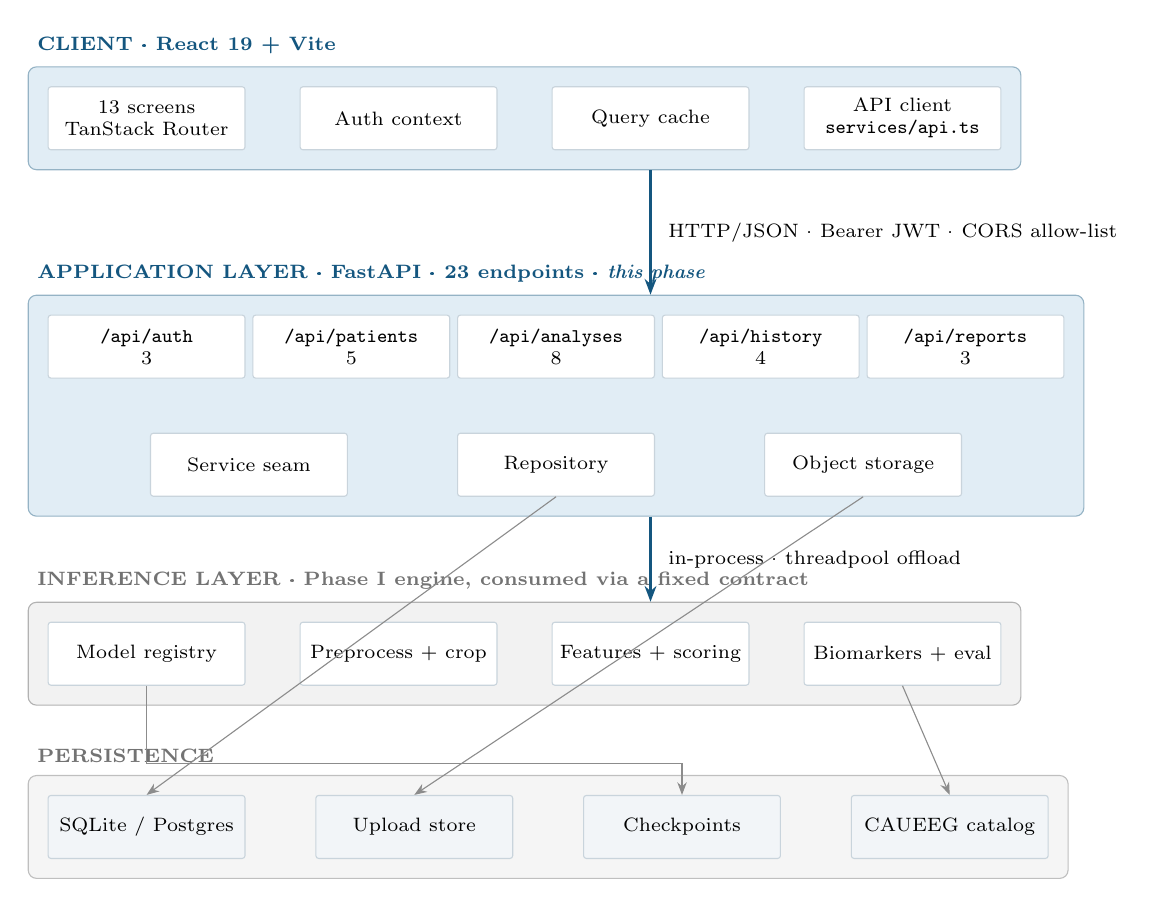
\begin{tikzpicture}[font=\scriptsize,
  box/.style={draw=rulegrey,fill=white,rounded corners=1pt,minimum height=8mm,
              minimum width=25mm,align=center,inner sep=2pt},
  store/.style={box,fill=softgrey},
  tier/.style={draw=accent!45,fill=accentlt,rounded corners=3pt,inner sep=7pt},
  lbl/.style={font=\scriptsize\bfseries,text=accent},
  arr/.style={-{Stealth[length=2mm]},draw=accent,thick},
  g/.style={-{Stealth[length=1.6mm]},draw=black!45}]

\node[box] (c1) at (0,0)   {13 screens\\TanStack Router};
\node[box] (c2) at (3.2,0) {Auth context};
\node[box] (c3) at (6.4,0) {Query cache};
\node[box] (c4) at (9.6,0) {API client\\\code{services/api.ts}};

\node[box] (a1) at (0,-2.9)   {\code{/api/auth}\\3};
\node[box] (a2) at (2.6,-2.9) {\code{/api/patients}\\5};
\node[box] (a3) at (5.2,-2.9) {\code{/api/analyses}\\8};
\node[box] (a4) at (7.8,-2.9) {\code{/api/history}\\4};
\node[box] (a5) at (10.4,-2.9){\code{/api/reports}\\3};
\node[box] (s1) at (1.3,-4.4) {Service seam};
\node[box] (s2) at (5.2,-4.4) {Repository};
\node[box] (s3) at (9.1,-4.4) {Object storage};

\node[box] (i1) at (0,-6.8)   {Model registry};
\node[box] (i2) at (3.2,-6.8) {Preprocess + crop};
\node[box] (i3) at (6.4,-6.8) {Features + scoring};
\node[box] (i4) at (9.6,-6.8) {Biomarkers + eval};

\node[store] (p1) at (0,-9.0)   {SQLite / Postgres};
\node[store] (p2) at (3.4,-9.0) {Upload store};
\node[store] (p3) at (6.8,-9.0) {Checkpoints};
\node[store] (p4) at (10.2,-9.0){CAUEEG catalog};

\begin{scope}[on background layer]
  \node[tier,fit=(c1)(c4)] (t1){}; \node[tier,fit=(a1)(a5)(s1)(s3)] (t2){};
  \node[tier,fit=(i1)(i4),fill=black!5,draw=black!30] (t3){};
  \node[tier,fit=(p1)(p4),fill=black!4,draw=black!25] (t4){};
\end{scope}
\node[lbl,anchor=south west] at ([yshift=1pt]t1.north west){CLIENT \textperiodcentered\ React 19 + Vite};
\node[lbl,anchor=south west] at ([yshift=1pt]t2.north west){APPLICATION LAYER \textperiodcentered\ FastAPI \textperiodcentered\ 23 endpoints \textperiodcentered\ \emph{this phase}};
\node[lbl,anchor=south west,text=black!55] at ([yshift=1pt]t3.north west){INFERENCE LAYER \textperiodcentered\ Phase I engine, consumed via a fixed contract};
\node[lbl,anchor=south west,text=black!55] at ([yshift=1pt]t4.north west){PERSISTENCE};

\draw[arr] (t1.south-|c3.center) -- node[right,font=\scriptsize]
  {\ HTTP/JSON \textperiodcentered\ Bearer JWT \textperiodcentered\ CORS allow-list} (t2.north-|c3.center);
\draw[arr] (t2.south-|c3.center) -- node[right,font=\scriptsize]
  {\ in-process \textperiodcentered\ threadpool offload} (t3.north-|c3.center);
\draw[g] (s2.south) -- (p1.north); \draw[g] (s3.south) -- (p2.north);
\draw[g] (i1.south) |- ([yshift=4mm]p3.north) -- (p3.north);
\draw[g] (i4.south) -- (p4.north);
\end{tikzpicture}}
\caption{Deployment architecture. The browser never addresses the inference
layer directly.}\label{fig:arch}
\end{figure}

\subsection{Use case diagram}

\begin{figure}[H]\centering
\resizebox{0.90\linewidth}{!}{%
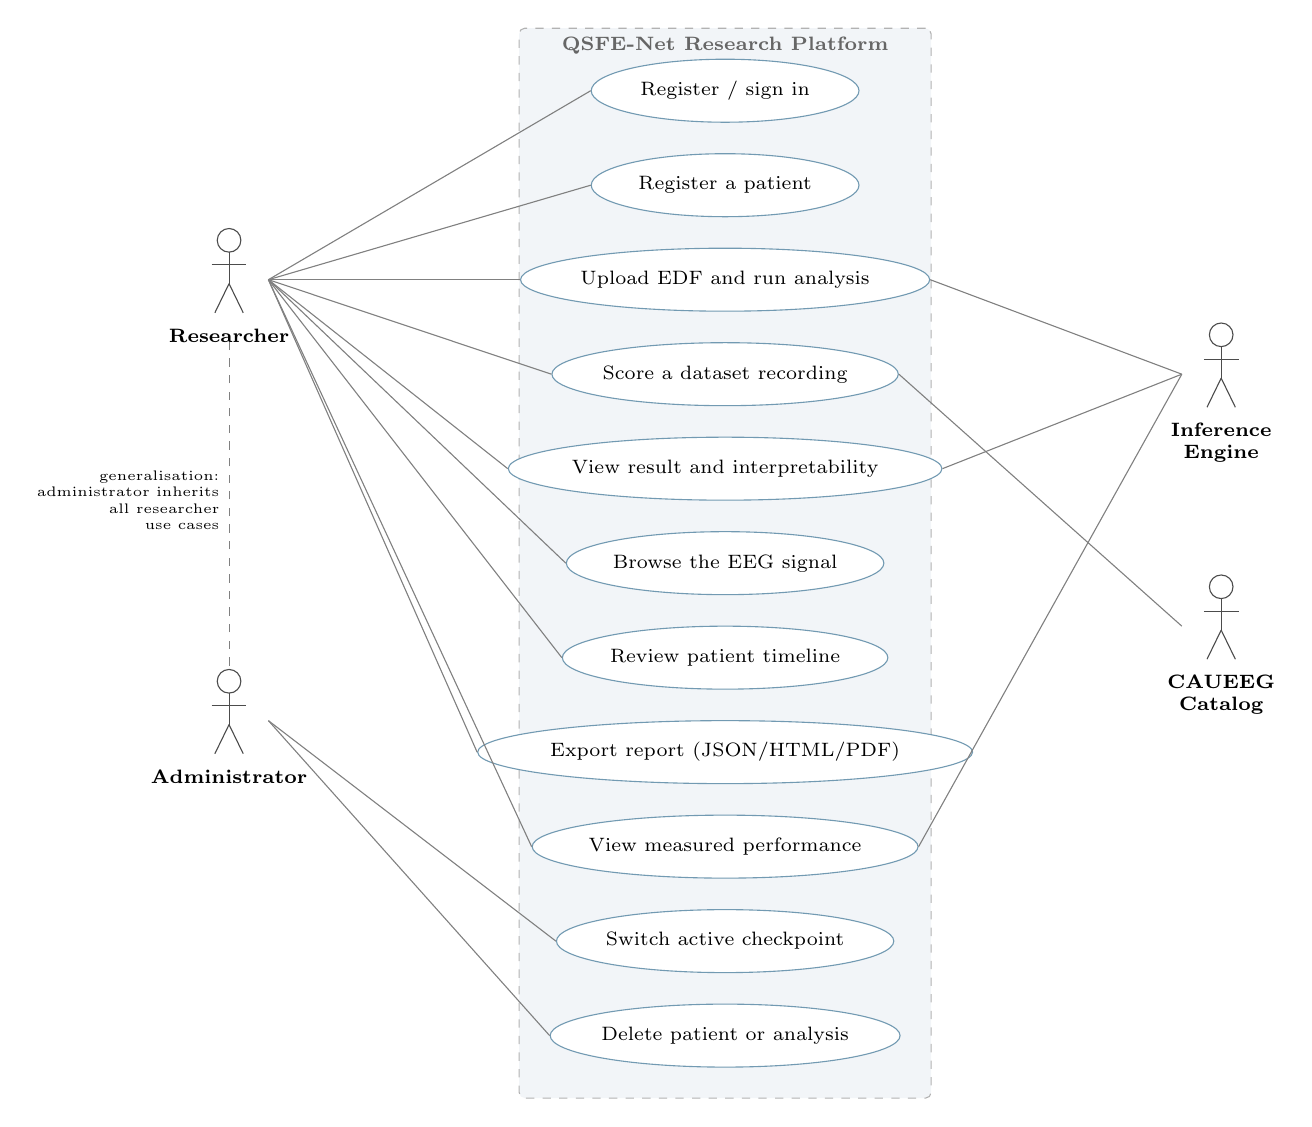
\begin{tikzpicture}[font=\scriptsize,
  uc/.style={draw=accent!60,fill=white,ellipse,minimum width=34mm,
             minimum height=8mm,align=center,inner sep=0pt},
  link/.style={draw=black!50}]
\newcommand{\actorfig}[3]{\begin{scope}[shift={(#1,#2)}]
  \draw[black!70] (0,.5) circle (.15); \draw[black!70] (0,.35)--(0,-.05);
  \draw[black!70] (-.22,.19)--(.22,.19); \draw[black!70] (0,-.05)--(-.18,-.42);
  \draw[black!70] (0,-.05)--(.18,-.42);
  \node[align=center,font=\scriptsize\bfseries,anchor=north] at (0,-.5){#3};\end{scope}}

\actorfig{0}{-3.0}{Researcher}
\actorfig{0}{-8.6}{Administrator}
\actorfig{12.6}{-4.2}{Inference\\Engine}
\actorfig{12.6}{-7.4}{CAUEEG\\Catalog}

\node[uc] (u1) at (6.3,-0.6) {Register / sign in};
\node[uc] (u2) at (6.3,-1.8) {Register a patient};
\node[uc] (u3) at (6.3,-3.0) {Upload EDF and run analysis};
\node[uc] (u4) at (6.3,-4.2) {Score a dataset recording};
\node[uc] (u5) at (6.3,-5.4) {View result and interpretability};
\node[uc] (u6) at (6.3,-6.6) {Browse the EEG signal};
\node[uc] (u7) at (6.3,-7.8) {Review patient timeline};
\node[uc] (u8) at (6.3,-9.0) {Export report (JSON/HTML/PDF)};
\node[uc] (u9) at (6.3,-10.2){View measured performance};
\node[uc] (u10)at (6.3,-11.4){Switch active checkpoint};
\node[uc] (u11)at (6.3,-12.6){Delete patient or analysis};

\begin{scope}[on background layer]
  \node[draw=black!30,dashed,rounded corners=2pt,fill=softgrey,
        fit=(u1)(u11),inner sep=11pt] (sys){};\end{scope}
\node[anchor=north,font=\scriptsize\bfseries,text=black!60] at (sys.north)
  {QSFE-Net Research Platform};

\foreach \n in {u1,u2,u3,u4,u5,u6,u7,u8,u9} \draw[link] (0.5,-3.0)--(\n.west);
\foreach \n in {u10,u11} \draw[link] (0.5,-8.6)--(\n.west);
\draw[link,dashed] (0,-7.9) -- node[left,font=\tiny,align=right]
  {generalisation:\\administrator inherits\\all researcher\\use cases} (0,-3.7);
\draw[link] (u3.east)--(12.1,-4.2); \draw[link] (u5.east)--(12.1,-4.2);
\draw[link] (u9.east)--(12.1,-4.2); \draw[link] (u4.east)--(12.1,-7.4);
\end{tikzpicture}}
\caption{Use case diagram.}\label{fig:uc}
\end{figure}

\subsection{Class diagram}

\begin{figure}[H]\centering
\resizebox{0.96\linewidth}{!}{%
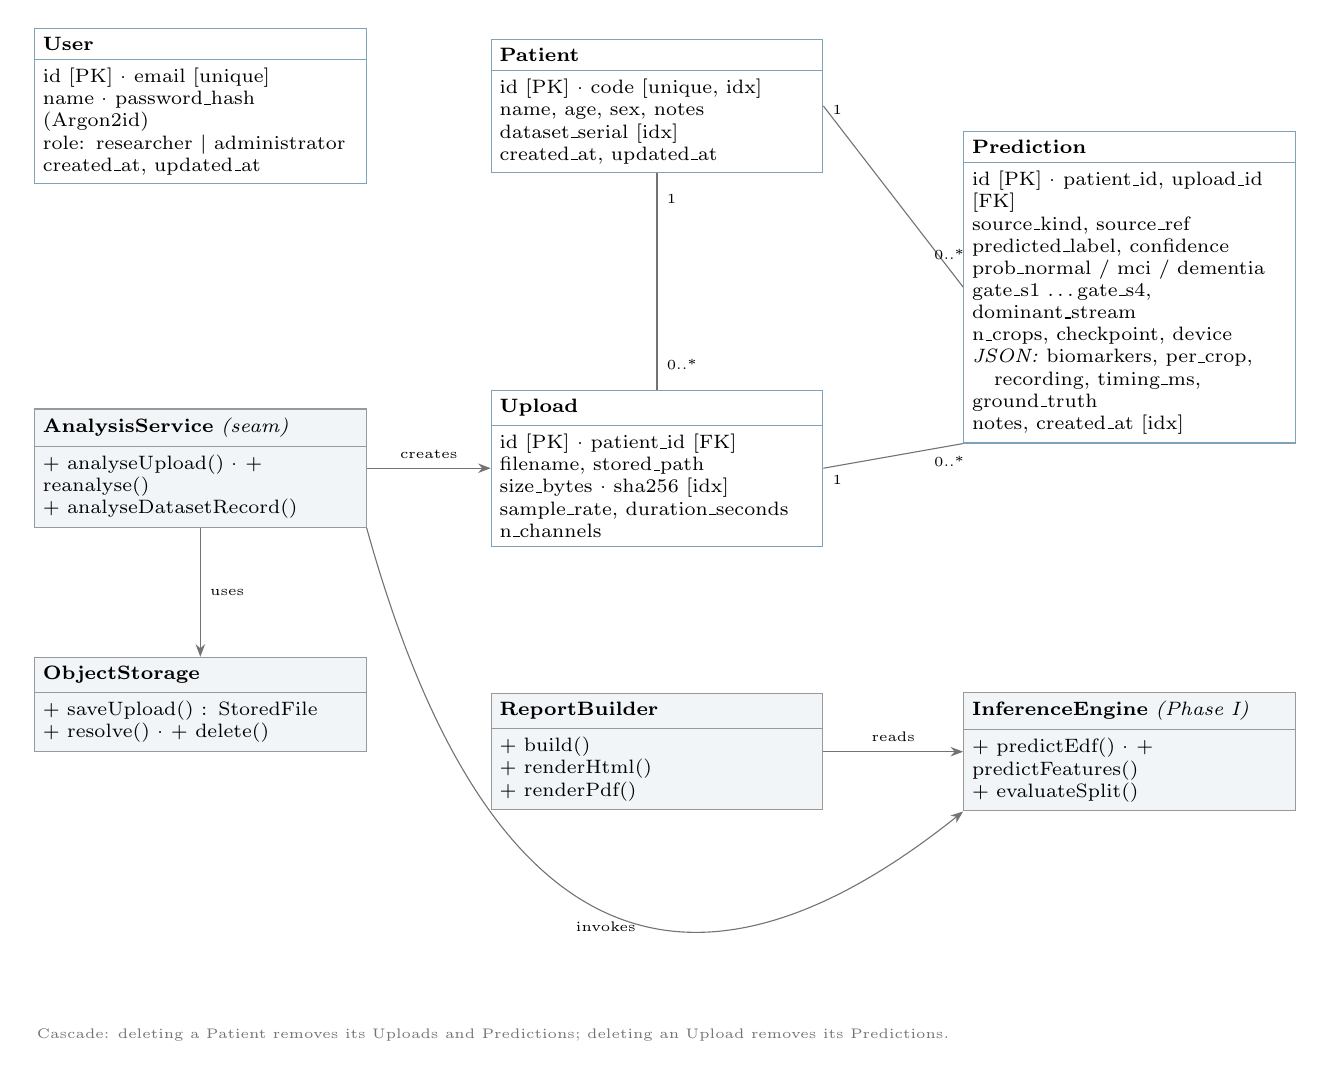
\begin{tikzpicture}[font=\scriptsize,
  cls/.style={draw=accent!55,fill=white,rectangle split,rectangle split parts=2,
              rectangle split part align=left,align=left,text width=40mm,inner sep=3pt},
  svc/.style={cls,draw=black!40,fill=softgrey},
  rel/.style={draw=black!55},
  arrw/.style={-{Stealth[length=1.6mm]},draw=black!55}]

\node[cls] (user) at (0,0) {\textbf{User}\nodepart{two}\raggedright
  id [PK] \textperiodcentered\ email [unique]\\ name \textperiodcentered\ password\_hash (Argon2id)\\
  role: researcher $|$ administrator\\ created\_at, updated\_at};

\node[cls] (pat) at (5.8,0) {\textbf{Patient}\nodepart{two}\raggedright
  id [PK] \textperiodcentered\ code [unique, idx]\\ name, age, sex, notes\\
  dataset\_serial [idx]\\ created\_at, updated\_at};

\node[cls] (up) at (5.8,-4.6) {\textbf{Upload}\nodepart{two}\raggedright
  id [PK] \textperiodcentered\ patient\_id [FK]\\ filename, stored\_path\\
  size\_bytes \textperiodcentered\ sha256 [idx]\\ sample\_rate, duration\_seconds\\ n\_channels};

\node[cls] (pred) at (11.8,-2.3) {\textbf{Prediction}\nodepart{two}\raggedright
  id [PK] \textperiodcentered\ patient\_id, upload\_id [FK]\\
  source\_kind, source\_ref\\
  predicted\_label, confidence\\
  prob\_normal / mci / dementia\\
  gate\_s1 \dots gate\_s4, dominant\_stream\\
  n\_crops, checkpoint, device\\
  \emph{JSON:} biomarkers, per\_crop,\\ \quad recording, timing\_ms, ground\_truth\\
  notes, created\_at [idx]};

\node[svc] (svc) at (0,-4.6) {\textbf{AnalysisService} \emph{(seam)}\nodepart{two}\raggedright
  + analyseUpload() \textperiodcentered\ + reanalyse()\\ + analyseDatasetRecord()};
\node[svc] (sto) at (0,-7.6) {\textbf{ObjectStorage}\nodepart{two}\raggedright
  + saveUpload() : StoredFile\\ + resolve() \textperiodcentered\ + delete()};
\node[svc] (rep) at (5.8,-8.2) {\textbf{ReportBuilder}\nodepart{two}\raggedright
  + build()\\ + renderHtml()\\ + renderPdf()};
\node[svc] (eng) at (11.8,-8.2) {\textbf{InferenceEngine} \emph{(Phase I)}\nodepart{two}\raggedright
  + predictEdf() \textperiodcentered\ + predictFeatures()\\ + evaluateSplit()};

\draw[rel] (pat.south)--node[right,font=\tiny,pos=.12]{1}node[right,font=\tiny,pos=.88]{0..*}(up.north);
\draw[rel] (pat.east)--node[above,font=\tiny,pos=.1]{1}node[above,font=\tiny,pos=.9]{0..*}(pred.west);
\draw[rel] (up.east)--node[below,font=\tiny,pos=.1]{1}node[below,font=\tiny,pos=.9]{0..*}(pred.south west);
\draw[arrw] (svc.east)--node[above,font=\tiny]{creates}(up.west);
\draw[arrw] (svc.south)--node[right,font=\tiny]{uses}(sto.north);
% Routed below ReportBuilder: a direct curve would cut straight through it.
\draw[arrw] (svc.south east) .. controls +(1.5,-5.4) and +(-3.5,-2.8) ..
  node[below,font=\tiny,pos=.5]{invokes}(eng.south west);
\draw[arrw] (rep.east)--node[above,font=\tiny]{reads}(eng.west);
\node[font=\tiny,text=black!55,align=left,anchor=north west] at (-2.2,-11.6)
  {Cascade: deleting a Patient removes its Uploads and Predictions; deleting an
   Upload removes its Predictions.};
\end{tikzpicture}}
\caption{Class diagram. Scalars that are filtered or aggregated are SQL columns;
bulky payloads are JSON columns beside them.}\label{fig:class}
\end{figure}

\subsection{Sequence diagram: upload and score}

\begin{figure}[H]\centering
\resizebox{0.95\linewidth}{!}{%
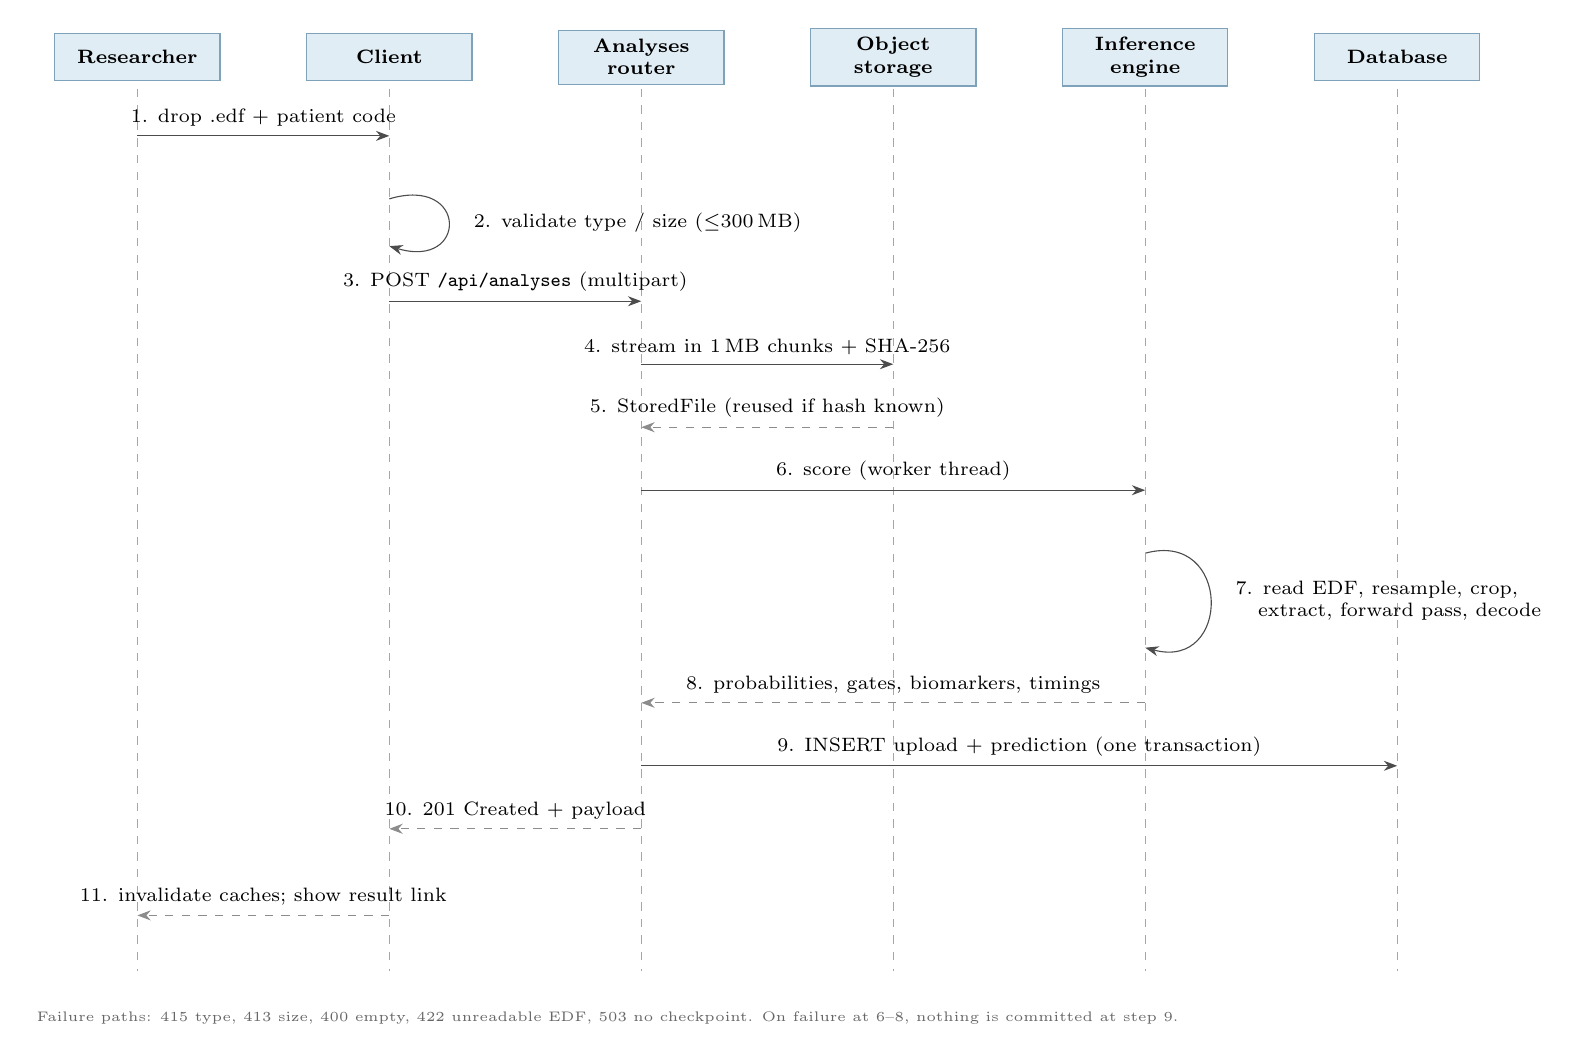
\begin{tikzpicture}[font=\scriptsize,
  head/.style={draw=accent!55,fill=accentlt,minimum width=21mm,minimum height=6mm,
               align=center,font=\scriptsize\bfseries},
  msg/.style={-{Stealth[length=1.7mm]},draw=black!70},
  ret/.style={-{Stealth[length=1.7mm]},draw=black!45,dashed}]
\def\A{0}\def\B{3.2}\def\C{6.4}\def\D{9.6}\def\E{12.8}\def\F{16.0}
\node[head](hA) at (\A,0){Researcher}; \node[head](hB) at (\B,0){Client};
\node[head](hC) at (\C,0){Analyses\\router}; \node[head](hD) at (\D,0){Object\\storage};
\node[head](hE) at (\E,0){Inference\\engine}; \node[head](hF) at (\F,0){Database};
\foreach \x in {\A,\B,\C,\D,\E,\F} \draw[dashed,black!35](\x,-0.4)--(\x,-11.6);

\draw[msg](\A,-1.0)--node[above]{1. drop .edf + patient code}(\B,-1.0);
\draw[msg](\B,-1.8) .. controls +(1,.3) and +(1,-.3) ..
  node[right,xshift=2mm]{2. validate type / size ($\le$300\,MB)}(\B,-2.4);
\draw[msg](\B,-3.1)--node[above]{3. POST \code{/api/analyses} (multipart)}(\C,-3.1);
\draw[msg](\C,-3.9)--node[above]{4. stream in 1\,MB chunks + SHA-256}(\D,-3.9);
\draw[ret](\D,-4.7)--node[above]{5. StoredFile (reused if hash known)}(\C,-4.7);
\draw[msg](\C,-5.5)--node[above]{6. score (worker thread)}(\E,-5.5);
\draw[msg](\E,-6.3) .. controls +(1.1,.3) and +(1.1,-.3) ..
  node[right,xshift=2mm,align=left]{7. read EDF, resample, crop,\\ \ \ \ extract, forward pass, decode}(\E,-7.5);
\draw[ret](\E,-8.2)--node[above]{8. probabilities, gates, biomarkers, timings}(\C,-8.2);
\draw[msg](\C,-9.0)--node[above]{9. INSERT upload + prediction (one transaction)}(\F,-9.0);
\draw[ret](\C,-9.8)--node[above]{10. 201 Created + payload}(\B,-9.8);
\draw[ret](\B,-10.9)--node[above]{11. invalidate caches; show result link}(\A,-10.9);
\node[align=left,font=\tiny,text=black!60,anchor=north west] at (-1.4,-12.0)
  {Failure paths: 415 type, 413 size, 400 empty, 422 unreadable EDF,
   503 no checkpoint. On failure at 6--8, nothing is committed at step~9.};
\end{tikzpicture}}
\caption{Sequence diagram for the principal use case.}\label{fig:seq}
\end{figure}

% ===================== 5. DESIGN =====================
\section{Design and Methodology}

\subsection{Proposed system}

Nine modules across four concerns. Figure~\ref{fig:blocks} is the block diagram;
Table~\ref{tab:modules} gives the technique adopted for each and its source.

\begin{figure}[H]\centering
\resizebox{0.95\linewidth}{!}{%
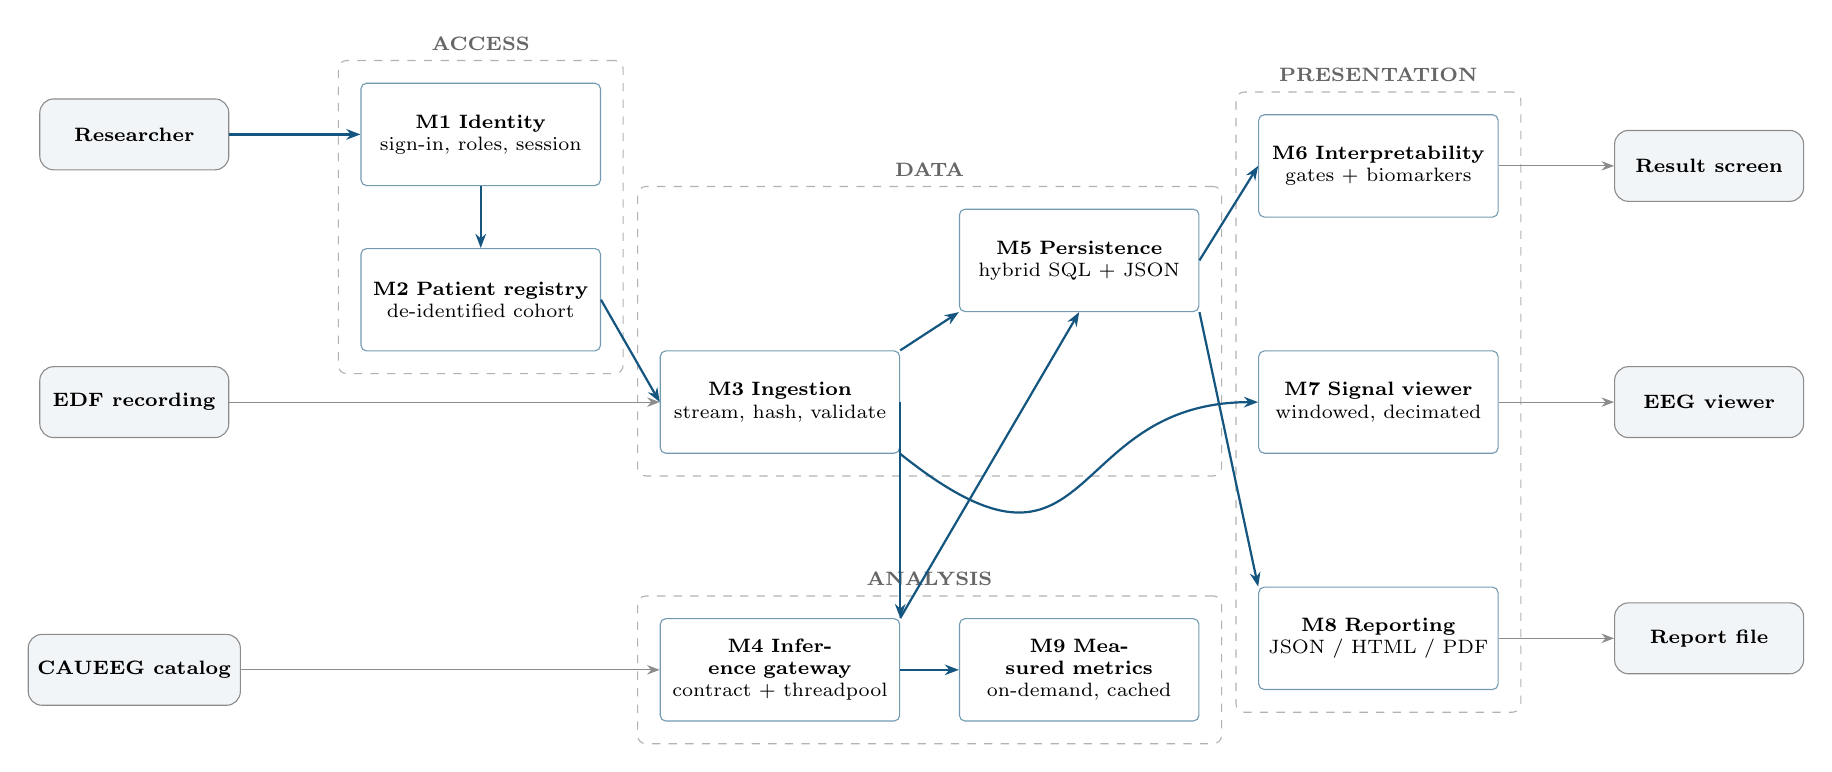
\begin{tikzpicture}[font=\scriptsize,
  mod/.style={draw=accent!60,fill=white,rounded corners=2pt,minimum width=30mm,
              minimum height=13mm,align=center,text width=29mm,inner sep=2pt},
  io/.style={draw=black!45,fill=softgrey,rounded corners=5pt,minimum width=24mm,
             minimum height=9mm,align=center},
  grp/.style={draw=black!30,dashed,rounded corners=3pt,inner sep=8pt},
  glbl/.style={font=\scriptsize\bfseries,text=black!60},
  f/.style={-{Stealth[length=1.8mm]},draw=accent,thick},
  g/.style={-{Stealth[length=1.6mm]},draw=black!45}]

\node[io](in1) at (-4.4,0){\textbf{Researcher}};
\node[io](in2) at (-4.4,-3.4){\textbf{EDF recording}};
\node[io](in3) at (-4.4,-6.8){\textbf{CAUEEG catalog}};

\node[mod](m1) at (0,0){\textbf{M1 Identity}\\sign-in, roles, session};
\node[mod](m2) at (0,-2.1){\textbf{M2 Patient registry}\\de-identified cohort};
\node[mod](m3) at (3.8,-3.4){\textbf{M3 Ingestion}\\stream, hash, validate};
\node[mod](m5) at (7.6,-1.6){\textbf{M5 Persistence}\\hybrid SQL + JSON};
\node[mod](m4) at (3.8,-6.8){\textbf{M4 Inference gateway}\\contract + threadpool};
\node[mod](m9) at (7.6,-6.8){\textbf{M9 Measured metrics}\\on-demand, cached};
\node[mod](m6) at (11.4,-0.4){\textbf{M6 Interpretability}\\gates + biomarkers};
\node[mod](m7) at (11.4,-3.4){\textbf{M7 Signal viewer}\\windowed, decimated};
\node[mod](m8) at (11.4,-6.4){\textbf{M8 Reporting}\\JSON / HTML / PDF};

\node[io](o1) at (15.6,-0.4){\textbf{Result screen}};
\node[io](o2) at (15.6,-3.4){\textbf{EEG viewer}};
\node[io](o3) at (15.6,-6.4){\textbf{Report file}};

\begin{scope}[on background layer]
 \node[grp,fit=(m1)(m2)](gA){}; \node[grp,fit=(m3)(m5)](gB){};
 \node[grp,fit=(m4)(m9)](gC){}; \node[grp,fit=(m6)(m8)](gD){};\end{scope}
\node[glbl,anchor=south] at (gA.north){ACCESS};
\node[glbl,anchor=south] at (gB.north){DATA};
\node[glbl,anchor=south] at (gC.north){ANALYSIS};
\node[glbl,anchor=south] at (gD.north){PRESENTATION};

\draw[f](in1)--(m1); \draw[g](in2)--(m3.west); \draw[g](in3)--(m4.west);
\draw[f](m1.south)--(m2.north); \draw[f](m2.east)--(m3.west);
\draw[f](m3.east)--(m4.north east); \draw[f](m4.east)--(m9.west);
\draw[f](m3.north east)--(m5.south west); \draw[f](m4.north east)--(m5.south);
\draw[f](m5.east)--(m6.west); \draw[f](m5.south east)--(m8.north west);
\draw[f](m3.south east) .. controls +(2.5,-2) and +(-2.5,0) .. (m7.west);
\draw[g](m6)--(o1); \draw[g](m7)--(o2); \draw[g](m8)--(o3);
\end{tikzpicture}}
\caption{Module block diagram.}\label{fig:blocks}
\end{figure}

\begin{table}[H]\centering
\caption{Module specifications: technique adopted and its source.}
\label{tab:modules}\scriptsize\renewcommand{\arraystretch}{1.15}
\begin{tabularx}{\linewidth}{@{}C{0.55cm} L{2.4cm} Y@{}}
\toprule
\textbf{ID} & \textbf{Module} & \textbf{Technique adopted} \\
\midrule
M1 & Identity \& session &
\textbf{Argon2id} password hashing with the reference default parameterisation
and rehash-on-login~\cite{biryukov2016}, chosen because memory-hardness resists
GPU-accelerated offline attack. \textbf{Stateless HS256 JWT}~\cite{rfc7519} with
the algorithm pinned at verification and a 12-hour lifetime; statelessness
follows Fielding's REST constraint~\cite{fielding2000}. Any 401 clears the token
centrally, and sign-in, registration and sign-out all clear the client query
cache so one user never sees another's cached cohort. \\
\addlinespace[2pt]
M2 & Patient registry &
CRUD over a de-identified entity (external code, age, sex, notes). A nullable
\code{dataset\_serial} links a row to a CAUEEG record~\cite{kim2023}, which is
what lets ground truth be shown for benchmark subjects and withheld for uploads
--- the evaluated/unevaluated distinction of~\cite{mitchell2019}. Writes are
idempotent by serial. \\
\addlinespace[2pt]
M3 & Ingestion &
(i) \emph{Streaming with incremental digest}: 1\,MB chunks written straight to
disk while SHA-256 updates in the same pass, so peak memory is one chunk and the
size cap is enforced mid-stream. (ii) \emph{Content addressing}: the file is
stored under a hash-derived path, so re-uploads deduplicate and any historical
result is re-derivable from the exact bytes~\cite{amershi2019}. (iii)
\emph{Format validation} per EDF/EDF+~\cite{kemp1992,kemp2003}. \\
\addlinespace[2pt]
M4 & Inference gateway &
A narrow contract --- recording or feature batch in; probabilities, gates,
biomarkers, metadata and timings out. Scoring is \emph{synchronous} but
dispatched to a worker thread because it is CPU-bound. The service function owns
``predict, then persist'' as one transaction, so no result is stored without
provenance and no failure leaves an orphan row. Checkpoint dimensions are read
from the file, not assumed~\cite{sculley2015}. \\
\addlinespace[2pt]
M5 & Persistence &
\textbf{Hybrid relational/document schema}~\cite{kleppmann2017}: filtered and
aggregated scalars (label, confidence, three probabilities, four gates, dominant
stream, checkpoint, timestamp) are typed columns; bulky always-read-together
payloads (biomarkers, per-crop, recording, timings, ground truth) are JSON. A
composite (patient, created\_at) index serves the timeline query. SQLite by
default, PostgreSQL confined to one schema for shared deployment; a startup
diagnostic performs a real round trip and warns loudly when running on SQLite,
because a host that wipes the container filesystem loses data silently while the
API still looks healthy. \\
\addlinespace[2pt]
M6 & Interpretability &
(i) \emph{Gate normalisation}: four raw activations shown as absolute weights
\emph{and} relative contributions, with the dominant stream named and worded as
contribution, not causation. (ii) \emph{Biomarker decoding}: the flat vector is
reshaped using fixed channel/band/pair orderings so ``element 7 of S1'' becomes
``delta power at F3''. No post-hoc surrogate is computed, following
Rudin~\cite{rudin2019}; decoding returns nothing rather than something wrong when
the layout does not match. \\
\addlinespace[2pt]
M7 & Signal viewer &
\emph{Server-side windowed decimation}: the client asks for a time window and a
point budget; only that window is read from the EDF and decimated per channel.
Samples are the source signal in native units, \emph{not} the normalised tensor
the model saw, and the response marks where the scored crops sit. Interaction
follows the grammar of MNE/EEGLAB~\cite{gramfort2013,delorme2004}. \\
\addlinespace[2pt]
M8 & Reporting &
One payload, three serialisers: JSON, a Jinja2~\cite{jinja} HTML template, and a
ReportLab~\cite{reportlab} PDF. All three carry the same disclaimer, checkpoint
identity, gate breakdown and biomarker summary --- the caveats cannot be
separated from the numbers, per~\cite{sendak2020}. \\
\addlinespace[2pt]
M9 & Measured metrics &
A \textbf{no-transcription policy}. Accuracy, macro-F1, the confusion matrix and
per-class metrics are computed on demand against the loaded checkpoint;
parameter count and device are read from it; the ablation table is parsed from
the file the training run wrote and labelled with the split it actually used.
Metrics are reported disaggregated by class~\cite{mitchell2019} and cached
\emph{keyed by checkpoint identity}, invalidated on reload~\cite{amershi2019}. \\
\bottomrule
\end{tabularx}
\end{table}

\subsection{Key design decisions}

\begin{table}[H]\centering\caption{Decisions, alternatives and rationale.}
\label{tab:dec}\scriptsize
\begin{tabularx}{\linewidth}{@{}L{2.7cm} L{2.9cm} Y@{}}
\toprule
\textbf{Decision} & \textbf{Alternative} & \textbf{Rationale} \\
\midrule
One process, two layers & Separate inference microservice & Avoids sending a
multi-megabyte recording over the wire twice; boundary kept explicit for later
extraction. \\
Synchronous scoring & Job queue with polling & A few seconds fits one request;
a queue adds broker, worker and job-state surface for no present benefit. \\
Stateless JWT & Server-side session table & Restart and replication without
invalidating sessions~\cite{fielding2000}; accepted cost is no early revocation,
mitigated by a 12-hour expiry. \\
Gate weights, no LIME/SHAP & Post-hoc attribution over 830 features & The gate
vector is a genuine internal quantity; a surrogate would be costly and confusable
with it~\cite{rudin2019}. \\
Fail with 503, never mock & Placeholder output when no checkpoint loads & A
plausible fake result is worse than an error in a research setting. \\
Single API client module & Per-component fetch calls & Prevents the undeclared
consumer debt pattern~\cite{sculley2015}. \\
\bottomrule
\end{tabularx}
\end{table}

\subsection{Security and degradation}

Argon2id credentials; pinned-algorithm expiring JWTs; roles gate destructive
operations; CORS restricted to an explicit allow-list; upload extension
allow-list, byte cap enforced during streaming, empty-file rejection and
temp-file cleanup on every failure path; a startup warning when the signing
secret is unset. A missing checkpoint, catalog or feature cache produces an
explicit attributed failure (503 with a diagnostic the interface renders) and
never a fabricated result --- a deliberate departure from a superseded prototype
in the repository whose mock mode derived predictions from a hash of the
filename.

% ===================== 6. IMPLEMENTATION =====================
\section{Implementation Details}

\subsection{Completion status}

\begin{table}[H]\centering\caption{Module-wise status. Weighted overall $\approx$82\%.}
\label{tab:status}\footnotesize
\begin{tabularx}{\linewidth}{@{}C{0.7cm} L{3.1cm} C{1.5cm} C{0.7cm} Y@{}}
\toprule
\textbf{ID} & \textbf{Module} & \textbf{Status} & \textbf{\%} & \textbf{Remaining} \\
\midrule
M1 & Identity \& session & \stDone & 100 & --- \\
M2 & Patient registry & \stDone & 100 & --- \\
M3 & Ingestion & \stPart & 90 & Compensating delete on failure (Obs.~3) \\
M4 & Inference gateway & \stPart & 85 & Asynchronous job path \\
M5 & Persistence & \stDone & 100 & --- \\
M6 & Interpretability & \stDone & 100 & --- \\
M7 & Signal viewer & \stPart & 80 & Amplitude scaling, stacked channels \\
M8 & Reporting & \stPart & 95 & Cohort-level export \\
M9 & Measured metrics & \stDone & 100 & Obs.~1 and Obs.~2 now fixed \\
\multicolumn{2}{@{}l}{Tests / CI} & \stPart & 40 & Two smoke suites; no unit tests \\
\multicolumn{2}{@{}l}{Deployment} & \stPart & 35 & No app container or CI \\
\multicolumn{2}{@{}l}{Accessibility} & \stTodo & 20 & Audit not yet performed \\
\bottomrule
\end{tabularx}
\end{table}

\subsection{Technical realisation}

The client is React~19 with file-based, fully typed TanStack routing --- a link
to a missing route is a compile error --- and all server state held in TanStack
Query, so a completed upload refreshes the dashboard, patient page and
prediction list through cache invalidation rather than hand-written propagation.
The server is FastAPI with SQLAlchemy~2.0 ORM models and Pydantic schemas at the
boundary, so the OpenAPI description is generated rather than written.

\begin{table}[H]\centering\caption{Delivered volume.}\label{tab:vol}\footnotesize
\begin{tabularx}{\linewidth}{@{}Y R{2.4cm}@{}}
\toprule \textbf{Measure} & \textbf{Value} \\ \midrule
Client modules / routed screens & 31 / 13 \\
Client application TypeScript (excl.\ 46 vendored UI primitives) & 5{,}965 LoC \\
Server application layer (this phase) & 2{,}248 LoC \\
HTTP endpoints, application layer / total surface & 23 / 36 \\
Persistent tables & 4 \\
Live workspace: users / patients & 3 / 15 \\
Live workspace: uploads / stored analyses & 5 / 14 \\
\bottomrule
\end{tabularx}
\end{table}

\subsection{Page-by-page walkthrough}
\label{sec:walk}

Every screenshot below was captured from a live instance
(\code{qsfe\_npz\_best.pth} on CUDA, 15 patients and 14 stored analyses)
using an automated browser at 1500\,px width. Table~\ref{tab:pages} summarises
what each screen does and the endpoints behind it; the figures follow.

\begin{table}[H]\centering\caption{Every screen, its function, and the endpoints behind it. The \code{/api} prefix is omitted in the last column.}
\label{tab:pages}\scriptsize\renewcommand{\arraystretch}{1.15}
\begin{tabularx}{\linewidth}{@{}L{2.5cm} C{0.7cm} Y L{3.5cm}@{}}
\toprule
\textbf{Route} & \textbf{LoC} & \textbf{What it does} & \textbf{Endpoints} \\
\midrule
\code{/login} & 178 & Credential entry; on success stores the JWT and clears any cached data from a previous session. Demo accounts are hinted inline. & \code{POST /auth/login} \\
\code{/register} & 79 & Account creation with a researcher/administrator role choice. & \code{POST /auth/register} \\
\code{/dashboard} & 438 & Workspace overview: analysis counts by predicted class, mean confidence, measured test accuracy and macro-F1, per-class metric bars, agreement with CAUEEG ground truth over labelled recordings only, mean gate weights by predicted class, an analyses-per-day trend, and recent activity. & \code{/history/stats} \newline \code{/history} \newline \code{/patients} \newline \code{/model/info} \newline \code{/model/performance} \\
\code{/patients} & 133 & Cohort registry: de-identified code, age, sex, analysis and upload counts, latest prediction, searchable. & \code{GET /patients} \\
\code{/patients/:id} & 352 & One subject: identifying fields, class-probability trajectory across sessions, distinct source recordings, gate-weight history, and the full analysis list. & \code{GET /patients/\{id\}} \newline \code{/history/patients/} \code{\{id\}/timeline} \\
\code{/upload} & 289 & Drag-and-drop EDF with client-side type and size validation, patient metadata form, a staged UPLOAD/PROCESSING/COMPLETED indicator, the inference pipeline described alongside, and a submit path gated on the live health check. & \code{POST /analyses} \newline \code{/health} \\
\code{/predictions} & 149 & Filterable history of every analysis: prediction, confidence, source kind, patient, timestamp. & \code{GET /history} \\
\code{/predictions/:id} & 451 & The interpretability report for one analysis: class probabilities, the four gate weights as relative stream contributions with the dominant stream named, decoded biomarkers per stream, provenance (checkpoint, device, crops, hash, timings) and JSON/HTML/PDF export. & \code{GET /analyses/\{id\}} \newline \code{/reports/\{id\}} \\
\code{/analysis} & 513 & EEG viewer over the source EDF with channel selection, zoom and pan, the scored crop windows shaded on the timeline, plus per-stream feature exploration and that stream's gate activation across the workspace. & \code{/analyses/\{id\}/} \code{waveform} \newline \code{GET /analyses/\{id\}} \\
\code{/model} & 281 & Architecture view with the forward pass laid out stream by stream, and measured gate analysis aggregated over stored analyses. & \code{/model/info} \newline \code{GET /history} \\
\code{/performance} & 411 & Confusion matrix, per-class precision/recall/F1/support, the ablation table labelled with the split it used, and published baselines marked as external. & \code{/model/performance} \newline \code{/model/ablation} \\
\code{/settings} & 250 & Account details, active model, checkpoint inventory with stream dimensions and extractor compatibility, and the resolved server environment. & \code{/model/checkpoints} \newline \code{POST /model/reload} \newline \code{/health} \\
\code{/about} & 179 & Scientific background, the four streams, and an explicit limitations section --- the platform's model-facts page~\cite{sendak2020}. & \code{/model/info} \newline \code{/model/performance} \\
\bottomrule
\end{tabularx}
\end{table}

\begin{figure}[H]\centering
\begin{minipage}[b]{0.485\linewidth}\centering
  \shot{01-login.png}\\[2pt]{\scriptsize (a) \code{/login}}
\end{minipage}\hfill
\begin{minipage}[b]{0.485\linewidth}\centering
  \shot{02-register.png}\\[2pt]{\scriptsize (b) \code{/register}}
\end{minipage}
\caption{\textbf{M1 --- Identity.} Credentials are verified against Argon2id
hashes and a 12-hour HS256 token is issued. Signing in clears the client query
cache so no cached record survives a user change.}\label{fig:auth}
\end{figure}

\begin{figure}[H]\centering
\shot[0.97\linewidth]{03-dashboard.png}
\caption{\textbf{M9 --- Dashboard.} Left group counts this workspace; right
group is the model measured on the held-out split. The 53.39\% accuracy, 0.5226
macro-F1 and the per-class bars are computed at request time from the active
checkpoint, not stored in the client. ``Agreement with CAUEEG truth'' is
deliberately restricted to the 9 of 14 analyses that have a verified label.}
\label{fig:dash}
\end{figure}

\begin{figure}[H]\centering
\begin{minipage}[b]{0.485\linewidth}\centering
  \shot{04-patients.png}\\[2pt]{\scriptsize (a) \code{/patients}}
\end{minipage}\hfill
\begin{minipage}[b]{0.485\linewidth}\centering
  \shot{07-predictions.png}\\[2pt]{\scriptsize (b) \code{/predictions}}
\end{minipage}
\caption{\textbf{M2, M5 --- Registry and history.} The cohort registry (a) and
the filterable analysis history (b). Both are ordinary SQL queries over the
typed columns of the hybrid schema.}\label{fig:lists}
\end{figure}

\begin{figure}[H]\centering
\shot[0.97\linewidth]{05-patient.png}
\caption{\textbf{M2 --- Patient record.} Class-probability trajectory across
sessions, distinct source recordings, and gate-weight history for one subject.
This is what makes repeat recordings a trajectory rather than unrelated
results.}\label{fig:patient}
\end{figure}

\begin{figure}[H]\centering
\shot[0.97\linewidth]{06-upload.png}
\caption{\textbf{M3, M4 --- New analysis.} Drag-and-drop ingestion with
client-side validation before any bytes are sent, patient metadata, a staged
status indicator, and the server-side pipeline described alongside. The panel at
lower right reads the live health endpoint and states the checkpoint and device
that will score the file.}\label{fig:upload}
\end{figure}

\begin{figure}[H]\centering
\shot[0.97\linewidth]{08-result.png}
\caption{\textbf{M6, M8 --- Result detail.} The case-first screen
Cai et al.~\cite{cai2019} argue for: probabilities, then the gate weights as
relative stream contributions, then biomarkers decoded to named electrodes and
bands, then provenance. Gate weights are labelled stream contribution, not
causal explanation.}\label{fig:result}
\end{figure}

\begin{figure}[H]\centering
\shot[0.97\linewidth]{09-analysis.png}
\caption{\textbf{M7 --- EEG viewer.} A 30\,s window of the source EDF read
server-side and decimated from 200\,Hz to 67\,Hz for display; the shaded band
marks where the scored crops sit. The caption states explicitly that these are
raw samples, not the z-normalised tensor the model consumed. Below, the selected
stream is described and its gate activation summarised across the
workspace.}\label{fig:viewer}
\end{figure}

\begin{figure}[H]\centering
\shot[0.97\linewidth]{11-performance.png}
\caption{\textbf{M9 --- Measured performance.} Confusion matrix and per-class
metrics computed by scoring all 118 test patients in 4.16\,s. Two corrections
from the verification pass are visible: ``Crops averaged 1 --- per recording,
5 requested'' (Obs.~2) and the ablation column now headed \textbf{Val acc} with
the hint ``validation accuracy, not test'' (Obs.~1).}\label{fig:perf}
\end{figure}

\begin{figure}[H]\centering
\shot[0.97\linewidth]{10-model.png}
\caption{\textbf{Architecture view.} The forward pass laid out stream by stream
with measured gate analysis. The figures come from \code{/model/info}, read out
of the loaded checkpoint rather than written into the page.}\label{fig:model}
\end{figure}

\begin{figure}[H]\centering
\begin{minipage}[b]{0.485\linewidth}\centering
  \shot{12-settings.png}\\[2pt]{\scriptsize (a) \code{/settings}}
\end{minipage}\hfill
\begin{minipage}[b]{0.485\linewidth}\centering
  \shot{13-about.png}\\[2pt]{\scriptsize (b) \code{/about}}
\end{minipage}
\caption{\textbf{M9 and model facts.} Settings (a) lists every checkpoint on
disk with its stream dimensions and whether it matches the current feature
extractor; switching one invalidates every cached metric. About (b) is the
model-facts page: background, the four streams, and an explicit limitations
section.}\label{fig:sysadmin}
\end{figure}

\clearpage
\subsection{Results, observations and analysis}

\textbf{Latency.} Timings are recorded per stage on every scored upload and
stored with the prediction, so Table~\ref{tab:lat} is read out of the workspace
database rather than measured separately. Device was CUDA.

\begin{table}[H]\centering\caption{Per-stage latency of the five scored uploads (ms), from stored provenance.}
\label{tab:lat}\footnotesize
\begin{tabular}{@{}l rrrr r@{}}
\toprule
\textbf{Crops} & \textbf{Cropping} & \textbf{Features} & \textbf{Forward pass} & \textbf{Total} & \textbf{Recording} \\
\midrule
3 & 32.6 & 2{,}618.4 & \phantom{0}73.5 & 2{,}728.6 & \phantom{0}728\,s \\
5 & \phantom{0}3.0 & 4{,}427.5 & 154.5 & 4{,}585.7 & 1{,}043\,s \\
5 & \phantom{0}2.9 & 4{,}067.3 & 110.4 & 4{,}181.1 & \phantom{0}651\,s \\
5 & \phantom{0}3.2 & 4{,}250.3 & 149.9 & 4{,}403.9 & 1{,}008\,s \\
5 & \phantom{0}3.6 & 3{,}787.2 & \phantom{0}17.5 & 3{,}812.1 & \phantom{0}847\,s \\
\midrule
\textbf{Mean (5 crops)} & \textbf{3.2} & \textbf{4{,}133.1} & \textbf{108.1} & \textbf{4{,}245.7} & \\
\bottomrule
\end{tabular}
\end{table}

\textbf{Observation A --- feature extraction dominates by two orders of
magnitude.} At five crops it is 97.3\% of wall-clock time, the forward pass
2.5\%, cropping 0.08\%. Per-crop extraction cost is 757--873\,ms across
recordings ranging from 651\,s to 1{,}043\,s, so cost scales with crop count, not
recording duration. Three consequences follow, all anticipated by the design.
The threadpool dispatch is justified --- a four-second CPU-bound block would
otherwise stall the event loop for every other request. GPU acceleration is
nearly irrelevant to perceived latency, because the expensive stage is SciPy
signal processing on the CPU: a faster GPU would improve the 2.5\% and leave the
97.3\% untouched. And the 16-crop maximum would take roughly 13\,s, which is past
the point where a request should be backgrounded --- this sets the threshold for
the asynchronous job path (T-21).

\textbf{Verification of M9.} Objective O6 requires that no displayed metric be a
transcription. The checkpoint was loaded independently, every patient in the
evaluation split was scored outside the application, and the result compared
with what the platform serves.

\begin{table}[H]\centering
\caption{Confusion matrix and per-class metrics served by the platform,
reproduced exactly by an independent recomputation.}
\label{tab:conf}\footnotesize
\begin{tabular}{@{}l rrr c rrrr@{}}
\toprule
& \multicolumn{3}{c}{\textbf{Predicted}} & & \multicolumn{4}{c}{\textbf{Per-class}} \\
\cmidrule(lr){2-4}\cmidrule(lr){6-9}
\textbf{True} & Normal & MCI & Dem. & & Prec. & Rec. & F1 & Supp. \\
\midrule
Normal   & \textbf{30} & 13 & 3  & & 0.6250 & 0.6522 & 0.6383 & 46 \\
MCI      & 12 & \textbf{20} & 9  & & 0.4444 & 0.4878 & 0.4651 & 41 \\
Dementia & 6  & 12 & \textbf{13} & & 0.5200 & 0.4194 & 0.4643 & 31 \\
\midrule
\multicolumn{9}{@{}l}{\textbf{Accuracy 53.39\%} \quad \textbf{Macro-F1 0.5226}
\quad (majority baseline 38.98\%; chance 33.3\%)} \\
\bottomrule
\end{tabular}
\end{table}

\textbf{Observation B --- the measured-metrics design works.} Accuracy,
macro-F1 and every confusion cell match to four decimal places, which is the
evidence for O6: the performance screen is derived from the checkpoint at
request time and cannot silently disagree with the weights on disk. Reporting
disaggregated by class~\cite{mitchell2019} also exposes what one accuracy figure
hides --- recall on Dementia (0.4194) is the weakest of the three despite that
class having the second-highest precision.

\begin{table}[H]\centering
\caption{Mean gate activation per stream over the 118 evaluated recordings.}
\label{tab:gates}\footnotesize
\begin{tabular}{@{}ll rr rrr@{}}
\toprule
& & \multicolumn{2}{c}{\textbf{Overall}} & \multicolumn{3}{c}{\textbf{By predicted class}} \\
\cmidrule(lr){3-4}\cmidrule(lr){5-7}
\textbf{Stream} & \textbf{Name} & Weight & Share & Normal & MCI & Dementia \\
\midrule
S1 & Frequency slowing & 0.7610 & 29.3\% & 0.7652 & 0.7650 & 0.7497 \\
S2 & Coherence & 0.9767 & 37.6\% & 0.9749 & 0.9778 & 0.9779 \\
S3 & Spectral entropy & 0.4534 & 17.5\% & 0.4976 & 0.4248 & 0.4256 \\
S4 & Hemispheric asymmetry & 0.4040 & 15.6\% & 0.4696 & 0.3874 & 0.3286 \\
\bottomrule
\end{tabular}
\end{table}

\textbf{Observation C --- the gate display is informative, not decorative.} The
gating is strongly non-uniform: coherence and slowing sit near saturation while
entropy and asymmetry are held to roughly 40--45\% of possible weight. Because
these are the network's own internal quantities rather than a post-hoc
attribution~\cite{rudin2019}, the display carries a genuine signal about what the
model relies on. S4 falls monotonically across predicted classes
(0.470 $\to$ 0.387 $\to$ 0.329) --- exactly the pattern the per-patient view
exists to let a researcher notice, which is the case-level behaviour
Cai et al.~\cite{cai2019} identified as the practitioner's real need. Explaining
\emph{why} the model weights streams this way is Phase~I territory.

\textbf{Observation D --- three defects found, two fixed.} These were recorded
rather than quietly patched, because two of them affect how results are
\emph{labelled} and are therefore reporting-integrity issues --- precisely the
class of problem the measured-metrics policy exists to prevent.

\begin{table}[H]\centering\caption{Defects found during verification and their resolution.}
\label{tab:def}\scriptsize\renewcommand{\arraystretch}{1.15}
\begin{tabularx}{\linewidth}{@{}C{0.5cm} L{3.0cm} Y C{1.1cm}@{}}
\toprule
\textbf{\#} & \textbf{Defect} & \textbf{Evidence and resolution} & \textbf{State} \\
\midrule
1 & The ablation table was served and displayed under the heading \emph{test
accuracy}, but the values are best \emph{validation} accuracy.
& The Phase~I ablation script builds only a train and a validation loader and
returns the best validation accuracy; the test split is never touched. The
served field was renamed to \code{val\_accuracy}, the finding text now says
``58.82\% validation'', and the column reads \textbf{Val acc} with the hint
``validation accuracy, not test'' (visible in Figure~\ref{fig:perf}).
& \stFixed \\
\addlinespace[2pt]
2 & The performance endpoint took a crop count defaulting to 5, implying five
crops were averaged per evaluated patient; only one cached crop exists per
evaluation patient, so the parameter was inert there.
& Cached feature files were counted per patient: all 118 evaluation patients
have exactly one crop, training patients have eight. The endpoint now records
the crops actually loaded and returns \code{n\_crops\_requested} alongside
\code{n\_crops}; the KPI reads ``1 --- per recording, 5 requested''. The
accuracy was never affected, only its description.
& \stFixed \\
\addlinespace[2pt]
3 & A recording is written to the content-addressed store before it is scored;
if scoring then fails, the file remains with no database row referencing it.
& One orphaned 32\,KB file was found in the upload store with no \code{uploads}
row, consistent with a malformed EDF that was stored and then failed header
validation. Fix scheduled as T-17: a compensating delete on the failure path
plus a sweep for unreferenced files.
& \stOpen \\
\bottomrule
\end{tabularx}
\end{table}

\textbf{Observation E --- silent data loss was designed out.} A startup
diagnostic performs a real database round trip rather than reporting
configuration, so a URL that is set but unreachable shows as disconnected
instead of appearing healthy. When the backend is SQLite it logs an explicit
non-persistence warning, because on a container host the file is wiped on every
restart while writes continue to succeed --- the failure mode where the API looks
healthy and the data is gone.

\textbf{Testing.} Two end-to-end smoke suites exist --- one over the inference
layer, one over the application layer against a throwaway database (registration,
sign-in, patient creation, an analysis run, history, all three report formats).
Both are run manually before each integration commit. There is no unit or
component coverage and no CI; that is the first task of next semester.

% ===================== 7. TECH STACK =====================
\section{Technology Stack}

\begin{figure}[H]\centering
\resizebox{0.97\linewidth}{!}{%
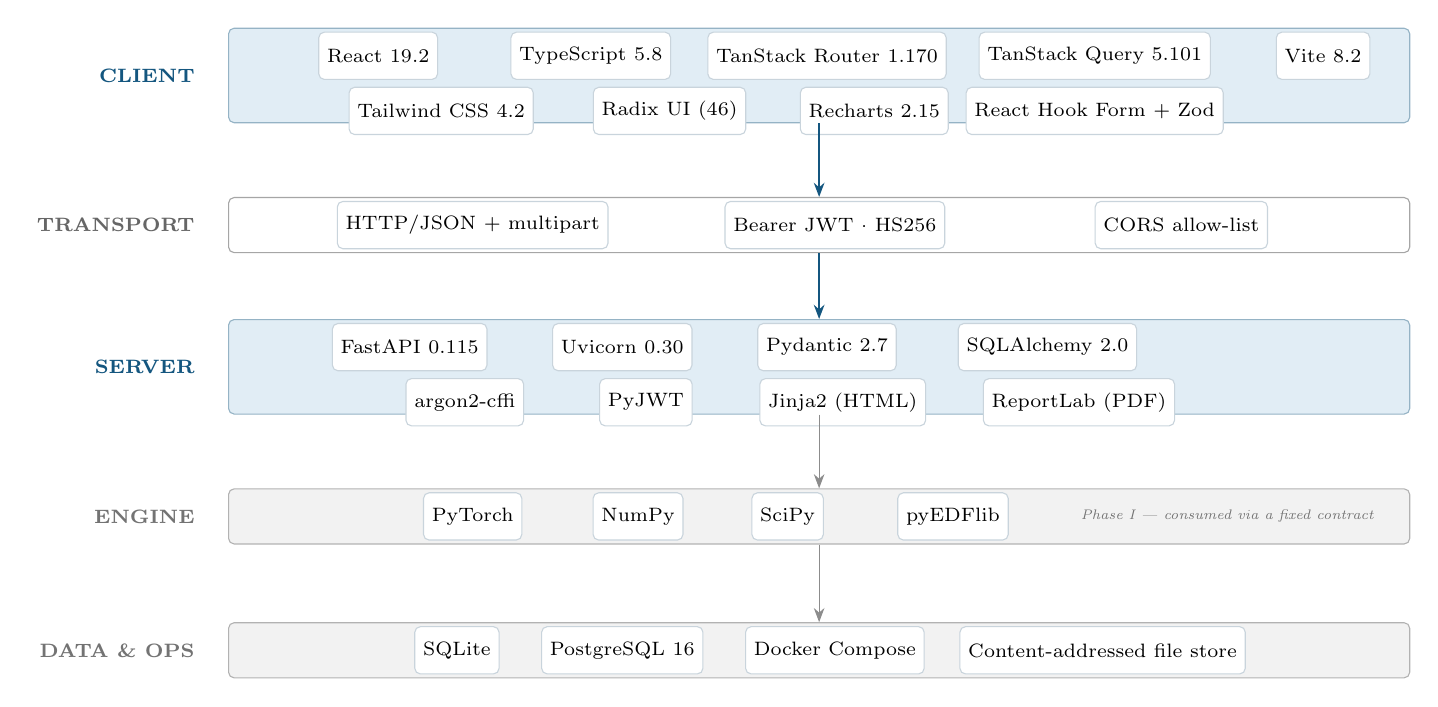
\begin{tikzpicture}[font=\scriptsize,
  lyr/.style={draw=accent!45,fill=accentlt,rounded corners=2pt,minimum width=150mm},
  chip/.style={draw=rulegrey,fill=white,rounded corners=2pt,minimum height=6mm,
               align=center,inner xsep=3pt,inner ysep=2pt},
  side/.style={font=\scriptsize\bfseries,text=accent,anchor=east},
  a/.style={-{Stealth[length=1.8mm]},draw=accent,thick}]

\node[lyr,minimum height=12mm](L1) at (0,0){}; \node[side] at ([xshift=-3mm]L1.west){CLIENT};
\node[chip] at (-5.6,.25){React 19.2}; \node[chip] at (-2.9,.25){TypeScript 5.8};
\node[chip] at (0.1,.25){TanStack Router 1.170}; \node[chip] at (3.5,.25){TanStack Query 5.101};
\node[chip] at (6.4,.25){Vite 8.2};
\node[chip] at (-4.8,-.45){Tailwind CSS 4.2}; \node[chip] at (-1.9,-.45){Radix UI (46)};
\node[chip] at (0.7,-.45){Recharts 2.15}; \node[chip] at (3.5,-.45){React Hook Form + Zod};

\node[lyr,minimum height=7mm,fill=white,draw=black!35](L2) at (0,-1.9){};
\node[side,text=black!60] at ([xshift=-3mm]L2.west){TRANSPORT};
\node[chip] at (-4.4,-1.9){HTTP/JSON + multipart};
\node[chip] at (0.2,-1.9){Bearer JWT \textperiodcentered\ HS256};
\node[chip] at (4.6,-1.9){CORS allow-list};

\node[lyr,minimum height=12mm](L3) at (0,-3.7){}; \node[side] at ([xshift=-3mm]L3.west){SERVER};
\node[chip] at (-5.2,-3.45){FastAPI 0.115}; \node[chip] at (-2.5,-3.45){Uvicorn 0.30};
\node[chip] at (0.1,-3.45){Pydantic 2.7}; \node[chip] at (2.9,-3.45){SQLAlchemy 2.0};
\node[chip] at (-4.5,-4.15){argon2-cffi}; \node[chip] at (-2.2,-4.15){PyJWT};
\node[chip] at (0.3,-4.15){Jinja2 (HTML)}; \node[chip] at (3.3,-4.15){ReportLab (PDF)};

\node[lyr,minimum height=7mm,fill=black!5,draw=black!30](L4) at (0,-5.6){};
\node[side,text=black!55] at ([xshift=-3mm]L4.west){ENGINE};
\node[chip] at (-4.4,-5.6){PyTorch}; \node[chip] at (-2.3,-5.6){NumPy};
\node[chip] at (-0.4,-5.6){SciPy}; \node[chip] at (1.7,-5.6){pyEDFlib};
\node[font=\tiny,text=black!55,anchor=west] at (3.2,-5.6){\emph{Phase I --- consumed via a fixed contract}};

\node[lyr,minimum height=7mm,fill=black!5,draw=black!30](L5) at (0,-7.3){};
\node[side,text=black!55] at ([xshift=-3mm]L5.west){DATA \& OPS};
\node[chip] at (-4.6,-7.3){SQLite}; \node[chip] at (-2.5,-7.3){PostgreSQL 16};
\node[chip] at (0.2,-7.3){Docker Compose}; \node[chip] at (3.6,-7.3){Content-addressed file store};

\draw[a](L1.south)--(L2.north); \draw[a](L2.south)--(L3.north);
\draw[-{Stealth[length=1.8mm]},black!45](L3.south)--(L4.north);
\draw[-{Stealth[length=1.8mm]},black!45](L4.south)--(L5.north);
\end{tikzpicture}}
\caption{Technology stack. Shaded layers are inherited from Phase~I or are
infrastructure; accented layers were built in this phase.}\label{fig:stack}
\end{figure}

\begin{table}[H]\centering\caption{Technologies, roles and references.}
\label{tab:tech}\scriptsize
\begin{tabularx}{\linewidth}{@{}L{2.5cm} C{1.25cm} Y L{1.3cm}@{}}
\toprule
\textbf{Technology} & \textbf{Version} & \textbf{Role} & \textbf{Ref.} \\
\midrule
React & 19.2 & Component model for all 13 screens & \cite{react} \\
TanStack Router / Query & 1.170 / 5.101 & Typed file-based routing; all server state, caching and invalidation & \cite{tanstack} \\
TypeScript & 5.8 & Static typing; the API client's types are the contract & \cite{typescript} \\
Tailwind CSS / Radix UI & 4.2 / --- & Styling tokens; 46 accessible unstyled primitives & \cite{tailwind,radix} \\
Recharts & 2.15 & Trajectories, gate histories, distributions & \cite{recharts} \\
Vite & 8.2 & Dev server and production bundling & \cite{vite} \\
FastAPI / Uvicorn & 0.115 / 0.30 & HTTP layer, DI, generated OpenAPI; ASGI server & \cite{fastapi,uvicorn} \\
Pydantic & 2.7 & Request/response validation; typed settings & \cite{pydantic} \\
SQLAlchemy & 2.0 & ORM, sessions, the hybrid schema & \cite{sqlalchemy} \\
argon2-cffi / PyJWT & 23.1 / 2.8 & Argon2id hashing; HS256 tokens (M1) & \cite{argon2cffi,pyjwt} \\
Jinja2 / ReportLab & 3.1 / 4.0 & HTML and PDF reports (M8) & \cite{jinja,reportlab} \\
SQLite / PostgreSQL & 3.x / 16 & Default and shared-deployment stores & \cite{sqlite,postgresql} \\
Docker Compose & --- & Optional local PostgreSQL & \cite{dockercompose} \\
PyTorch, NumPy, SciPy, pyEDFlib & --- & Phase~I engine: forward pass, arrays, signal processing, EDF I/O & \cite{paszke2019,harris2020,virtanen2020,pyedflib} \\
Playwright & --- & Automated capture of the screenshots in Section~\ref{sec:walk} & \cite{playwright} \\
PGF/TikZ, pgfgantt & --- & All diagrams and the timeline in this report & \cite{tikz,pgfgantt} \\
\bottomrule
\end{tabularx}
\end{table}

\textbf{Why these.} FastAPI was chosen over Flask because Pydantic declares the
request and response contracts once and enforces them automatically, the OpenAPI
description is generated so documentation cannot drift from the implementation,
and the ASGI foundation supplies the threadpool offload the CPU-bound scoring
path needs (Observation~A). TanStack Query was chosen over Redux because the
platform has almost no client state --- nearly everything on screen is a cached
projection of server state. SQLAlchemy with a SQLite default lets a researcher
clone and run the platform with no database service while the same code targets
PostgreSQL for shared deployment.

% ===================== 8. PLAN =====================
\section{Project Plan and Timeline}

\begin{figure}[H]\centering
\resizebox{0.97\linewidth}{!}{%
\begin{ganttchart}[hgrid,vgrid,x unit=8mm,y unit title=7mm,y unit chart=5.6mm,
  title height=1,title label font=\scriptsize\bfseries,
  group label font=\scriptsize\bfseries,bar label font=\scriptsize,
  milestone label font=\scriptsize\itshape,
  bar/.append style={fill=accent!70,draw=accent},
  bar incomplete/.append style={fill=accent!22,draw=accent!50},
  group/.append style={fill=black!55,draw=black!55},
  milestone/.append style={fill=warnamber,draw=warnamber}]{1}{10}
\gantttitle{Semester VII \textperiodcentered\ Phase II}{8}
\gantttitle{Sem VIII}{2} \\
\gantttitle{Jun}{1}\gantttitle{Jul}{2}\gantttitle{Aug}{2}\gantttitle{Sep}{1}
\gantttitle{Oct}{1}\gantttitle{Nov}{1}\gantttitle{Jan--Apr}{2} \\
\ganttgroup{Requirements and design}{1}{3} \\
\ganttbar[progress=100]{T-01 Requirements, scope boundary}{1}{1} \\
\ganttbar[progress=100]{T-02 Literature survey (platform)}{1}{2} \\
\ganttbar[progress=100]{T-03 Architecture, UML, schema}{2}{3} \\
\ganttgroup{Core implementation}{2}{6} \\
\ganttbar[progress=100]{T-04 M1 identity, M2 registry}{2}{3} \\
\ganttbar[progress=100]{T-05 M5 persistence}{3}{4} \\
\ganttbar[progress=90]{T-06 M3 ingestion, object store}{3}{4} \\
\ganttbar[progress=85]{T-07 M4 inference gateway}{4}{5} \\
\ganttbar[progress=100]{T-08 M6 interpretability}{4}{5} \\
\ganttbar[progress=80]{T-09 M7 signal viewer}{5}{6} \\
\ganttbar[progress=95]{T-10 M8 reporting}{5}{6} \\
\ganttbar[progress=100]{T-11 M9 measured metrics}{5}{6} \\
\ganttgroup{Integration, verification, reporting}{6}{8} \\
\ganttbar[progress=100]{T-12 Frontend--backend integration}{6}{7} \\
\ganttbar[progress=100]{T-13 Verification pass, defect log}{7}{7} \\
\ganttbar[progress=100]{T-14 Obs.~1 and Obs.~2 fixes}{7}{8} \\
\ganttbar[progress=80]{T-15 Phase II report}{7}{8} \\
\ganttmilestone{Phase II review}{8} \\
\ganttgroup{Planned}{9}{10} \\
\ganttbar[progress=0]{T-17--T-28 next semester}{9}{10}
\end{ganttchart}}
\caption{Timeline. Bar fill shows progress as of this report.}\label{fig:gantt}
\end{figure}

\begin{table}[H]\centering\caption{Module-wise plan for next semester.}
\label{tab:next}\footnotesize
\begin{tabularx}{\linewidth}{@{}C{0.9cm} C{1.25cm} Y L{1.4cm}@{}}
\toprule
\textbf{Task} & \textbf{Module} & \textbf{Description} & \textbf{Target} \\
\midrule
\multicolumn{4}{@{}l}{\emph{Block A --- close the last correctness gap}} \\
T-17 & M3 & Compensating delete on post-storage failure; sweep for unreferenced files (Obs.~3) & Jan wk 1 \\
\multicolumn{4}{@{}l}{\emph{Block B --- test coverage}} \\
T-18 & all & Unit tests for repository, report renderers, storage, auth; 70\% line coverage target & Jan--Feb \\
T-19 & client & Component tests for upload flow, result screen, auth context & Feb \\
T-20 & --- & CI pipeline: lint, type-check, both suites on every push & Feb wk 2 \\
\multicolumn{4}{@{}l}{\emph{Block C --- scalability and operations}} \\
T-21 & M4 & Asynchronous job path (submit returns a job id), justified by the 4.2\,s mean and 13\,s worst case in Table~\ref{tab:lat} & Feb--Mar \\
T-22 & M3, M4 & Profile and optimise feature extraction --- 97.3\% of request time & Mar \\
T-23 & --- & Application container and single-command compose stack; Postgres deployment so data is persistent (Obs.~E); register the engine repository properly & Mar \\
\multicolumn{4}{@{}l}{\emph{Block D --- capability and evaluation}} \\
T-24 & M7 & Viewer completion: amplitude scaling, stacked channels, montage re-referencing & Mar \\
T-25 & M6 & Optional SHAP~\cite{lundberg2017} attribution view, visually separated from the genuine gates and labelled an approximation~\cite{rudin2019} & Mar--Apr \\
T-26 & M2, M3 & EEG-BIDS conformant import/export~\cite{pernet2019} & Apr \\
T-27 & --- & Usability study (5--8 domain users) against Nielsen's heuristics~\cite{nielsen1994} and the onboarding needs of~\cite{cai2019}; accessibility audit across all 13 screens & Apr \\
T-28 & --- & Security review, final report and demonstration & Apr--May \\
\bottomrule
\end{tabularx}
\end{table}

\textbf{Risks.} The asynchronous path (T-21) could regress the working
synchronous flow --- mitigated by keeping synchronous as the default behind a
flag until Block~B coverage exists. Optimising feature extraction (T-22) could
change numerical output --- mitigated by a golden-file regression test asserting
bit-comparable vectors. The attribution view (T-25) could be misread as ground
truth --- mitigated by visual separation and explicit labelling.

% ===================== 9. REFERENCES =====================
\section{References}

{\footnotesize
% thebibliography emits its own \section*{References}; we already have a
% numbered section heading, so swallow the internal one.
\let\qsfeoldsection\section
\renewcommand{\section}[2]{}
\begin{thebibliography}{99}\setlength{\itemsep}{2pt}

\bibitem{amershi2019} Amershi, S., Begel, A., Bird, C., DeLine, R., Gall, H., Kamar, E., Nagappan, N., Nushi, B., and Zimmermann, T. (2019). ``Software Engineering for Machine Learning: A Case Study.'' \emph{Proc. ICSE-SEIP}, IEEE, pp.~291--300.

\bibitem{argon2cffi} argon2-cffi. \emph{Argon2 for Python}. \url{https://argon2-cffi.readthedocs.io/}

\bibitem{biryukov2016} Biryukov, A., Dinu, D., and Khovratovich, D. (2016). ``Argon2: New Generation of Memory-Hard Functions for Password Hashing and Other Applications.'' \emph{Proc. IEEE EuroS\&P}, pp.~292--302.

\bibitem{cai2019} Cai, C. J., Winter, S., Steiner, D., Wilcox, L., and Terry, M. (2019). ``\,`Hello AI': Uncovering the Onboarding Needs of Medical Practitioners for Human-AI Collaborative Decision-Making.'' \emph{PACM on Human-Computer Interaction}, 3(CSCW), Article~104.

\bibitem{delorme2004} Delorme, A., and Makeig, S. (2004). ``EEGLAB: an open source toolbox for analysis of single-trial EEG dynamics including independent component analysis.'' \emph{J. Neuroscience Methods}, 134(1), pp.~9--21.

\bibitem{dockercompose} Docker Inc. \emph{Docker Compose Documentation}. \url{https://docs.docker.com/compose/}

\bibitem{fastapi} Ram\'irez, S. \emph{FastAPI Documentation}. \url{https://fastapi.tiangolo.com/}

\bibitem{fielding2000} Fielding, R. T. (2000). \emph{Architectural Styles and the Design of Network-based Software Architectures}. Doctoral dissertation, University of California, Irvine.

\bibitem{gramfort2013} Gramfort, A., Luessi, M., Larson, E., et al. (2013). ``MEG and EEG data analysis with MNE-Python.'' \emph{Frontiers in Neuroscience}, 7:267.

\bibitem{harris2020} Harris, C. R., Millman, K. J., van der Walt, S. J., et al. (2020). ``Array programming with NumPy.'' \emph{Nature}, 585, pp.~357--362.

\bibitem{jinja} Pallets Projects. \emph{Jinja Template Engine Documentation}. \url{https://jinja.palletsprojects.com/}

\bibitem{rfc7519} Jones, M., Bradley, J., and Sakimura, N. (2015). \emph{JSON Web Token (JWT)}. RFC 7519, IETF. \url{https://www.rfc-editor.org/rfc/rfc7519}

\bibitem{kelly2019} Kelly, C. J., Karthikesalingam, A., Suleyman, M., Corrado, G., and King, D. (2019). ``Key challenges for delivering clinical impact with artificial intelligence.'' \emph{BMC Medicine}, 17:195.

\bibitem{kemp1992} Kemp, B., V\"arri, A., Rosa, A. C., Nielsen, K. D., and Gade, J. (1992). ``A simple format for exchange of digitized polygraphic recordings.'' \emph{Electroencephalography and Clinical Neurophysiology}, 82(5), pp.~391--393.

\bibitem{kemp2003} Kemp, B., and Olivan, J. (2003). ``European data format `plus' (EDF+), an EDF alike standard format for the exchange of physiological data.'' \emph{Clinical Neurophysiology}, 114(9), pp.~1755--1761.

\bibitem{kim2023} Kim, M., Youn, Y. C., and Paik, J. (2023). ``Deep learning-based EEG analysis to classify normal, mild cognitive impairment, and dementia: Algorithms and dataset.'' \emph{NeuroImage}, 272, 120054.

\bibitem{kleppmann2017} Kleppmann, M. (2017). \emph{Designing Data-Intensive Applications}. O'Reilly Media.

\bibitem{lundberg2017} Lundberg, S. M., and Lee, S.-I. (2017). ``A Unified Approach to Interpreting Model Predictions.'' \emph{NeurIPS 30}, pp.~4765--4774.

\bibitem{mitchell2019} Mitchell, M., Wu, S., Zaldivar, A., et al. (2019). ``Model Cards for Model Reporting.'' \emph{Proc. ACM FAT*}, pp.~220--229.

\bibitem{nielsen1994} Nielsen, J. (1994). ``Enhancing the explanatory power of usability heuristics.'' \emph{Proc. ACM CHI '94}, pp.~152--158.

\bibitem{paszke2019} Paszke, A., Gross, S., Massa, F., et al. (2019). ``PyTorch: An Imperative Style, High-Performance Deep Learning Library.'' \emph{NeurIPS 32}, pp.~8024--8035.

\bibitem{pernet2019} Pernet, C. R., Appelhoff, S., Gorgolewski, K. J., et al. (2019). ``EEG-BIDS, an extension to the brain imaging data structure for electroencephalography.'' \emph{Scientific Data}, 6:103.

\bibitem{pgfgantt} Wielath, W., and Isemann, M. \emph{The pgfgantt Package}. CTAN. \url{https://ctan.org/pkg/pgfgantt}

\bibitem{playwright} Microsoft. \emph{Playwright: browser automation library}. \url{https://playwright.dev/}

\bibitem{postgresql} PostgreSQL Global Development Group. \emph{PostgreSQL 16 Documentation}. \url{https://www.postgresql.org/docs/16/}

\bibitem{pydantic} Colvin, S., et al. \emph{Pydantic Documentation}. \url{https://docs.pydantic.dev/}

\bibitem{pyedflib} Nahrstaedt, H., and Lee-Messer, C. \emph{pyEDFlib Documentation}. \url{https://pyedflib.readthedocs.io/}

\bibitem{pyjwt} Padilla, J. \emph{PyJWT Documentation}. \url{https://pyjwt.readthedocs.io/}

\bibitem{radix} Radix UI. \emph{Radix Primitives Documentation}. \url{https://www.radix-ui.com/primitives}

\bibitem{react} Meta Open Source. \emph{React Documentation}. \url{https://react.dev/}

\bibitem{recharts} Recharts. \emph{Recharts Documentation}. \url{https://recharts.org/}

\bibitem{reportlab} ReportLab. \emph{ReportLab PDF Toolkit Documentation}. \url{https://docs.reportlab.com/}

\bibitem{ribeiro2016} Ribeiro, M. T., Singh, S., and Guestrin, C. (2016). ``\,`Why Should I Trust You?': Explaining the Predictions of Any Classifier.'' \emph{Proc. ACM SIGKDD}, pp.~1135--1144.

\bibitem{rudin2019} Rudin, C. (2019). ``Stop explaining black box machine learning models for high stakes decisions and use interpretable models instead.'' \emph{Nature Machine Intelligence}, 1, pp.~206--215.

\bibitem{sculley2015} Sculley, D., Holt, G., Golovin, D., et al. (2015). ``Hidden Technical Debt in Machine Learning Systems.'' \emph{NeurIPS 28}, pp.~2503--2511.

\bibitem{sendak2020} Sendak, M. P., Gao, M., Brajer, N., and Balu, S. (2020). ``Presenting machine learning model information to clinical end users with model facts labels.'' \emph{npj Digital Medicine}, 3:41.

\bibitem{shneiderman2020} Shneiderman, B. (2020). ``Human-Centered Artificial Intelligence: Reliable, Safe \& Trustworthy.'' \emph{Int. J. Human--Computer Interaction}, 36(6), pp.~495--504.

\bibitem{sqlalchemy} Bayer, M. \emph{SQLAlchemy 2.0 Documentation}. \url{https://docs.sqlalchemy.org/en/20/}

\bibitem{sqlite} SQLite Consortium. \emph{SQLite Documentation}. \url{https://www.sqlite.org/docs.html}

\bibitem{tailwind} Tailwind Labs. \emph{Tailwind CSS Documentation}. \url{https://tailwindcss.com/docs}

\bibitem{tanstack} Potter, T., et al. \emph{TanStack Router and Query Documentation}. \url{https://tanstack.com/}

\bibitem{tikz} Tantau, T. \emph{The TikZ and PGF Packages Manual}. CTAN. \url{https://ctan.org/pkg/pgf}

\bibitem{typescript} Microsoft. \emph{TypeScript Documentation}. \url{https://www.typescriptlang.org/docs/}

\bibitem{uvicorn} Christie, T., et al. \emph{Uvicorn Documentation}. \url{https://www.uvicorn.org/}

\bibitem{virtanen2020} Virtanen, P., Gommers, R., Oliphant, T. E., et al. (2020). ``SciPy 1.0: fundamental algorithms for scientific computing in Python.'' \emph{Nature Methods}, 17, pp.~261--272.

\bibitem{vite} You, E., et al. \emph{Vite Documentation}. \url{https://vite.dev/}

\end{thebibliography}
\let\section\qsfeoldsection}

\end{document}
